
\chapter{}
\label{sec:Appendix}
% Hier greift man einige wenige, interessante Gesichtspunkte der
% Implementierung heraus. Das Kapitel darf nicht mit Dokumentation oder
% gar Programmkommentaren verwechselt werden. Es kann vorkommen, daß
% sehr viele Gesichtspunkte aufgegriffen werden müssen, ist aber nicht
% sehr häufig. Zweck dieses Kapitels ist einerseits, glaubhaft zu
% machen, daß man es bei der Arbeit nicht mit einem "Papiertiger"
% sondern einem real existierenden System zu tun hat. Es ist sicherlich
% auch ein sehr wichtiger Text für jemanden, der die Arbeit später
% fortsetzt. Der dritte Gesichtspunkt dabei ist, einem Leser einen etwas
% tieferen Einblick in die Technik zu geben, mit der man sich hier
% beschäftigt. Schöne Bespiele sind "War Stories", also Dinge mit denen
% man besonders zu kämpfen hatte, oder eine konkrete, beispielhafte
% Verfeinerung einer der in Kapitel 3 vorgestellten Ideen. Auch hier
% gilt, mehr als 20 Seiten liest keiner, aber das ist hierbei nicht so
% schlimm, weil man die Lektüre ja einfach abbrechen kann, ohne den
% Faden zu verlieren. Vollständige Quellprogramme haben in einer Arbeit
% nichts zu suchen, auch nicht im Anhang, sondern gehören auf Rechner,
% auf denen man sie sich ansehen kann.
\begin{figure}[H]
  \centering
  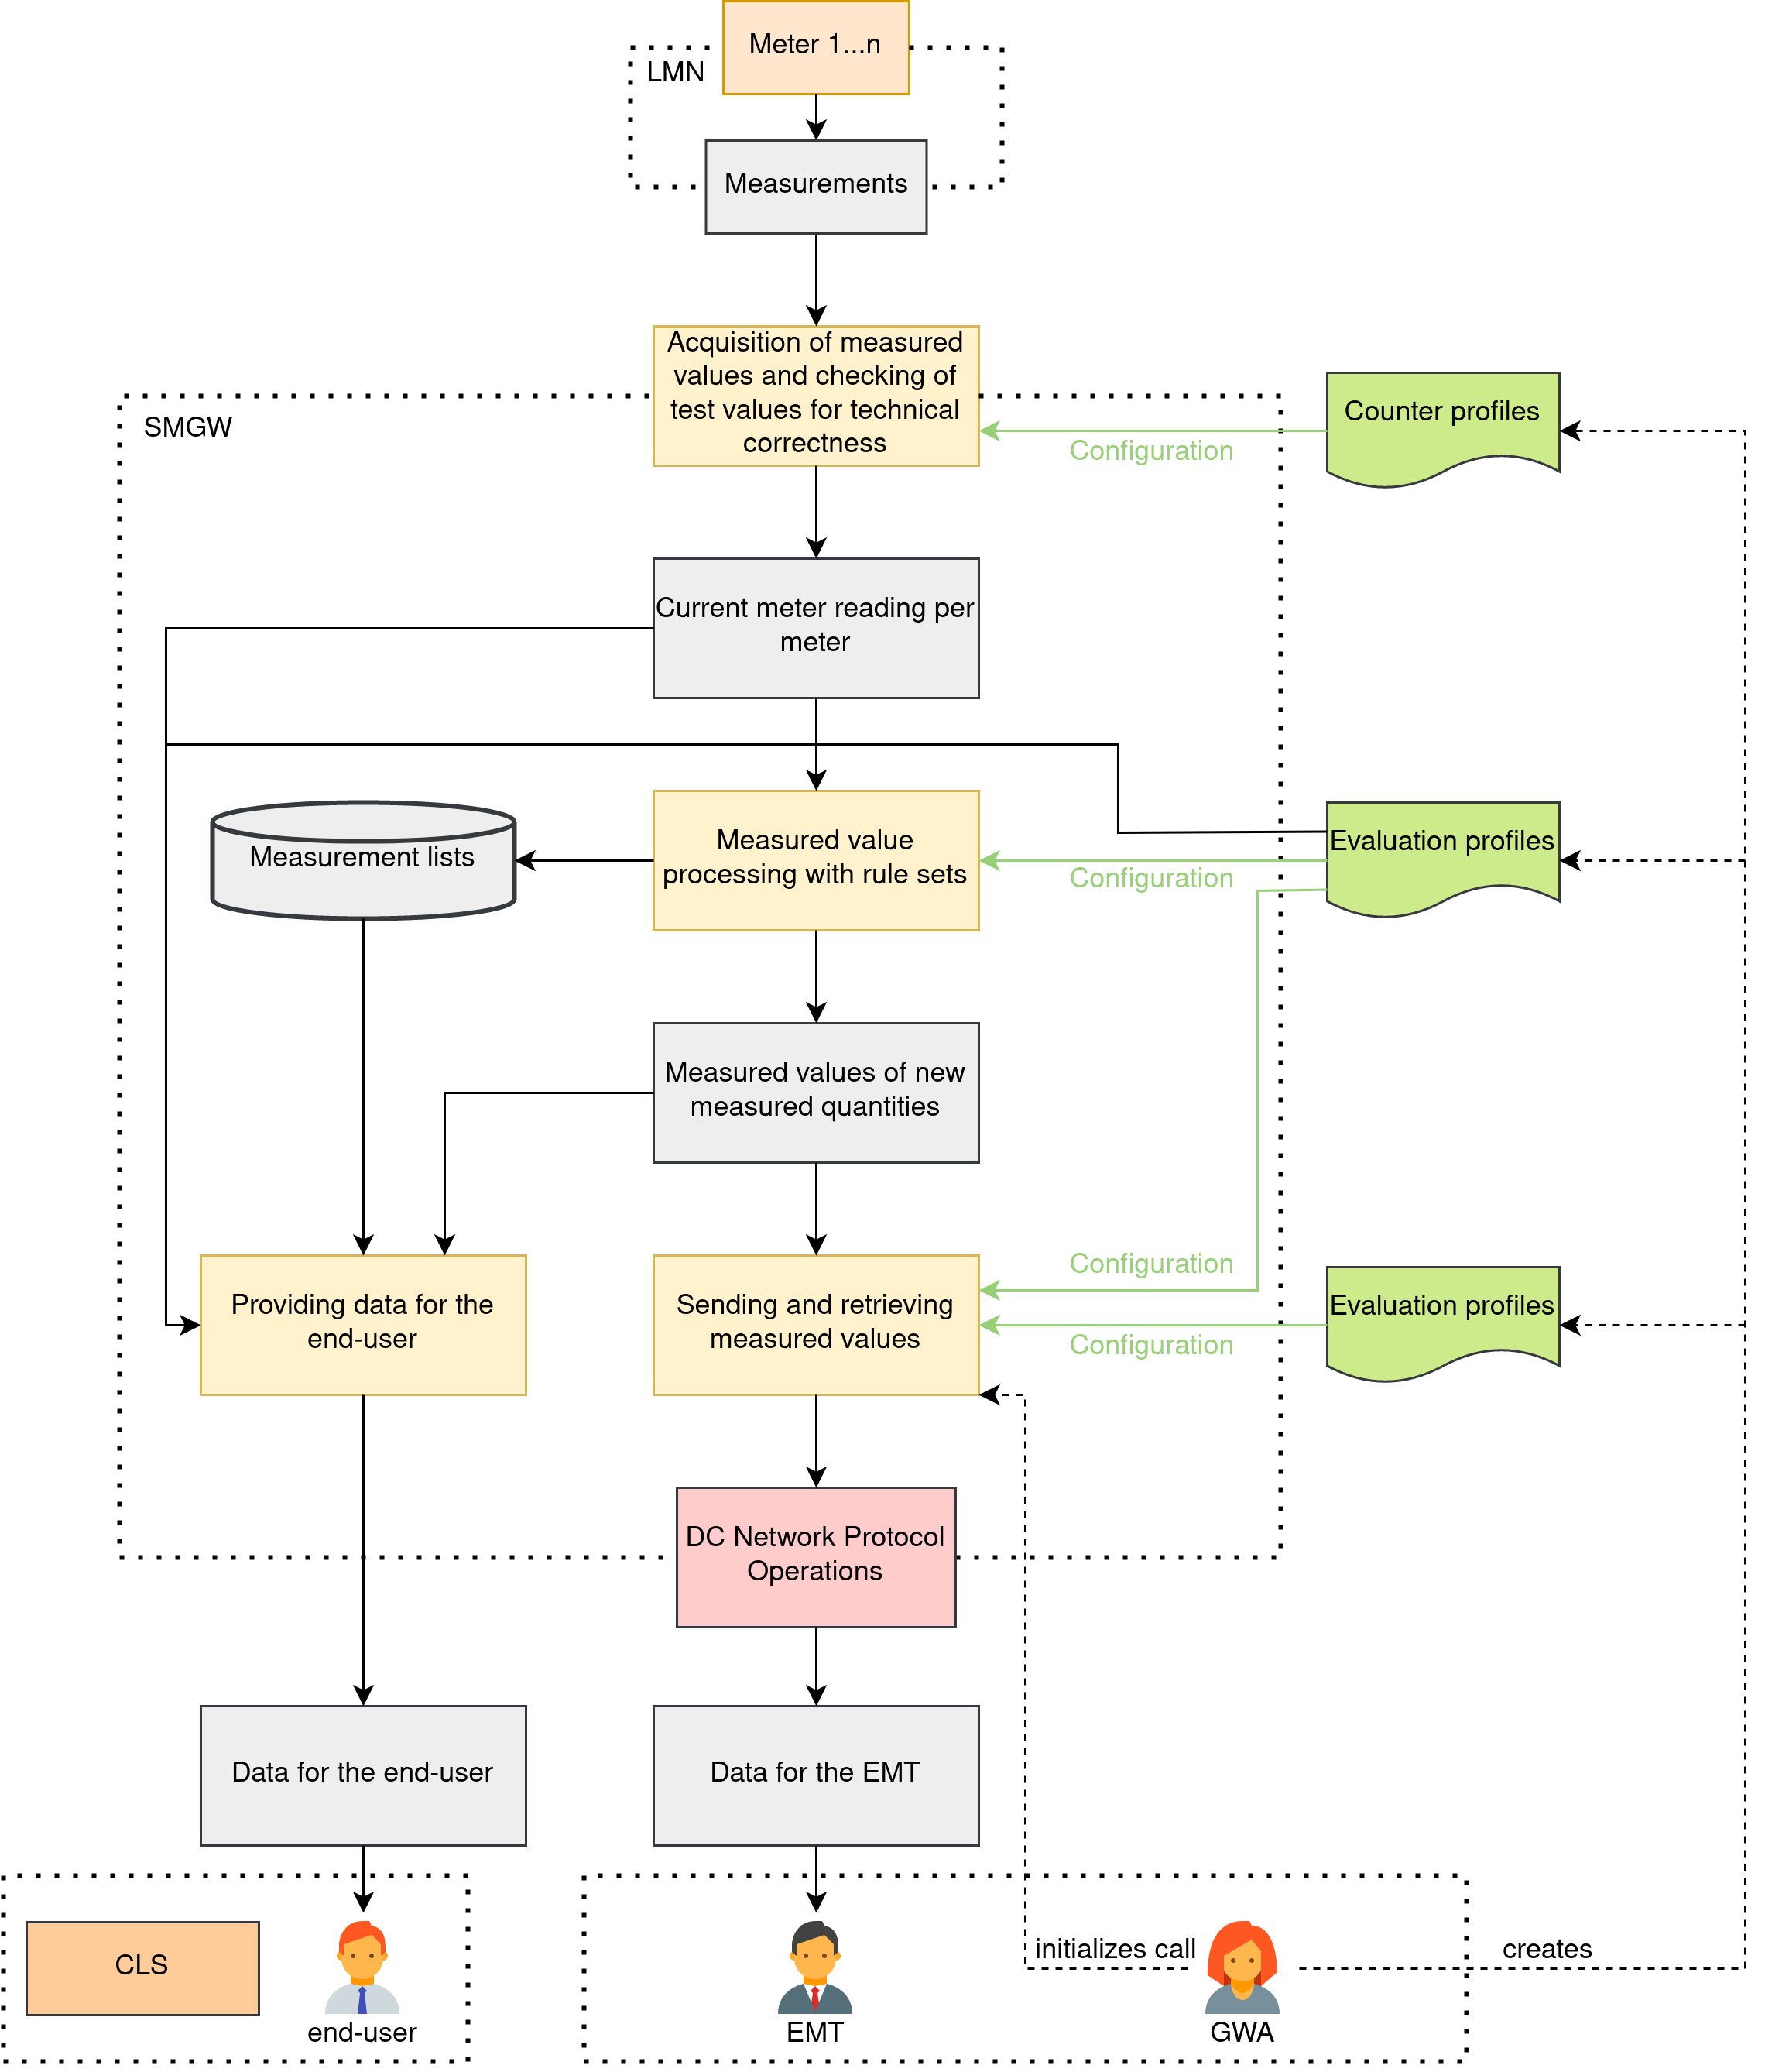
\includegraphics[width=1\textwidth]{images/Messverarbeitung_mit_DC_Eng2.png}
  \caption[Measured Value Processing in a SMGW]{An overview of the measured value processing within the SMGW with configuration profiles from the GWA and DC Network Protocol Extension.}
  \label{fig:value_processing_with_dc}
\end{figure}
%\renewcommand\topfraction{1}   
%\renewcommand\floatpagefraction{1}
\chapter{Two Weeks Experiments}
\enlargethispage{10}
\vspace*{-10\baseline}
\begin{figure}[!Hhtp]
\centering
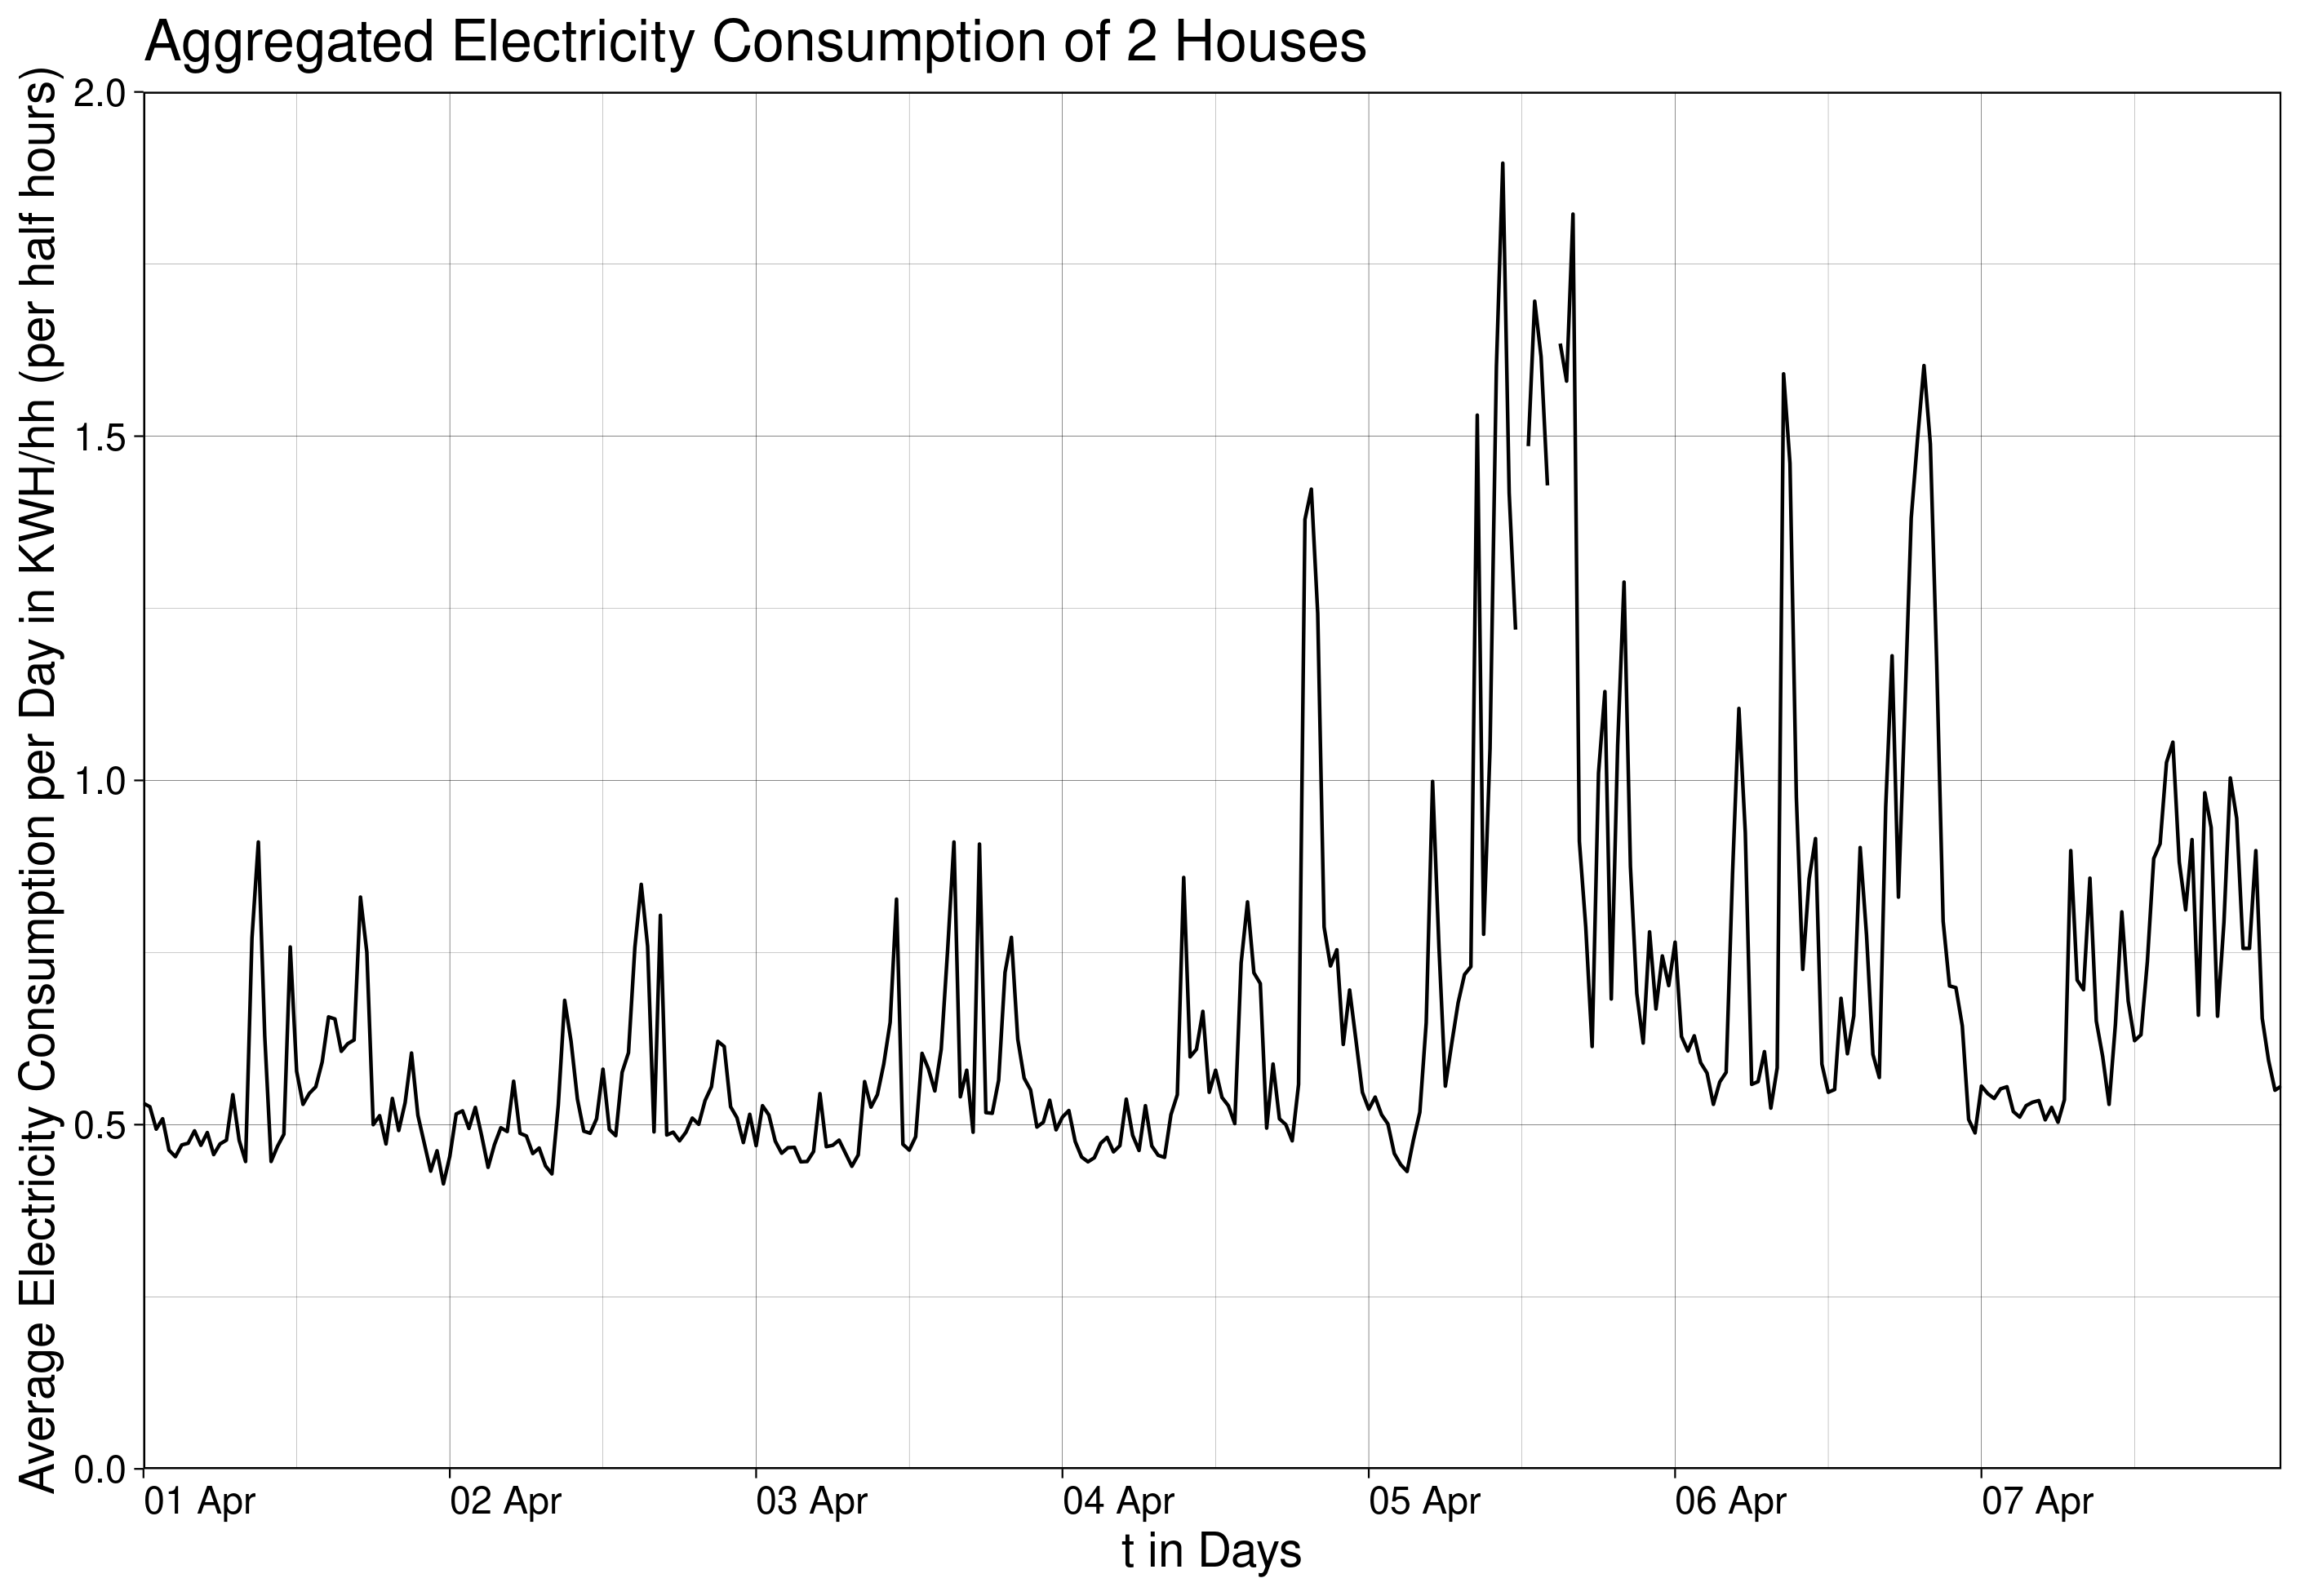
\includegraphics[width=0.8\columnwidth]{images/Aggregated Electricity Consumption of 2 Houses6.png}
\caption[Aggregated Electricity Consumption of 2 Houses of the 2nd Experiment]{}
\label{img:2_Houses_weekly}
%\vspace*{\floatsep}
\centering
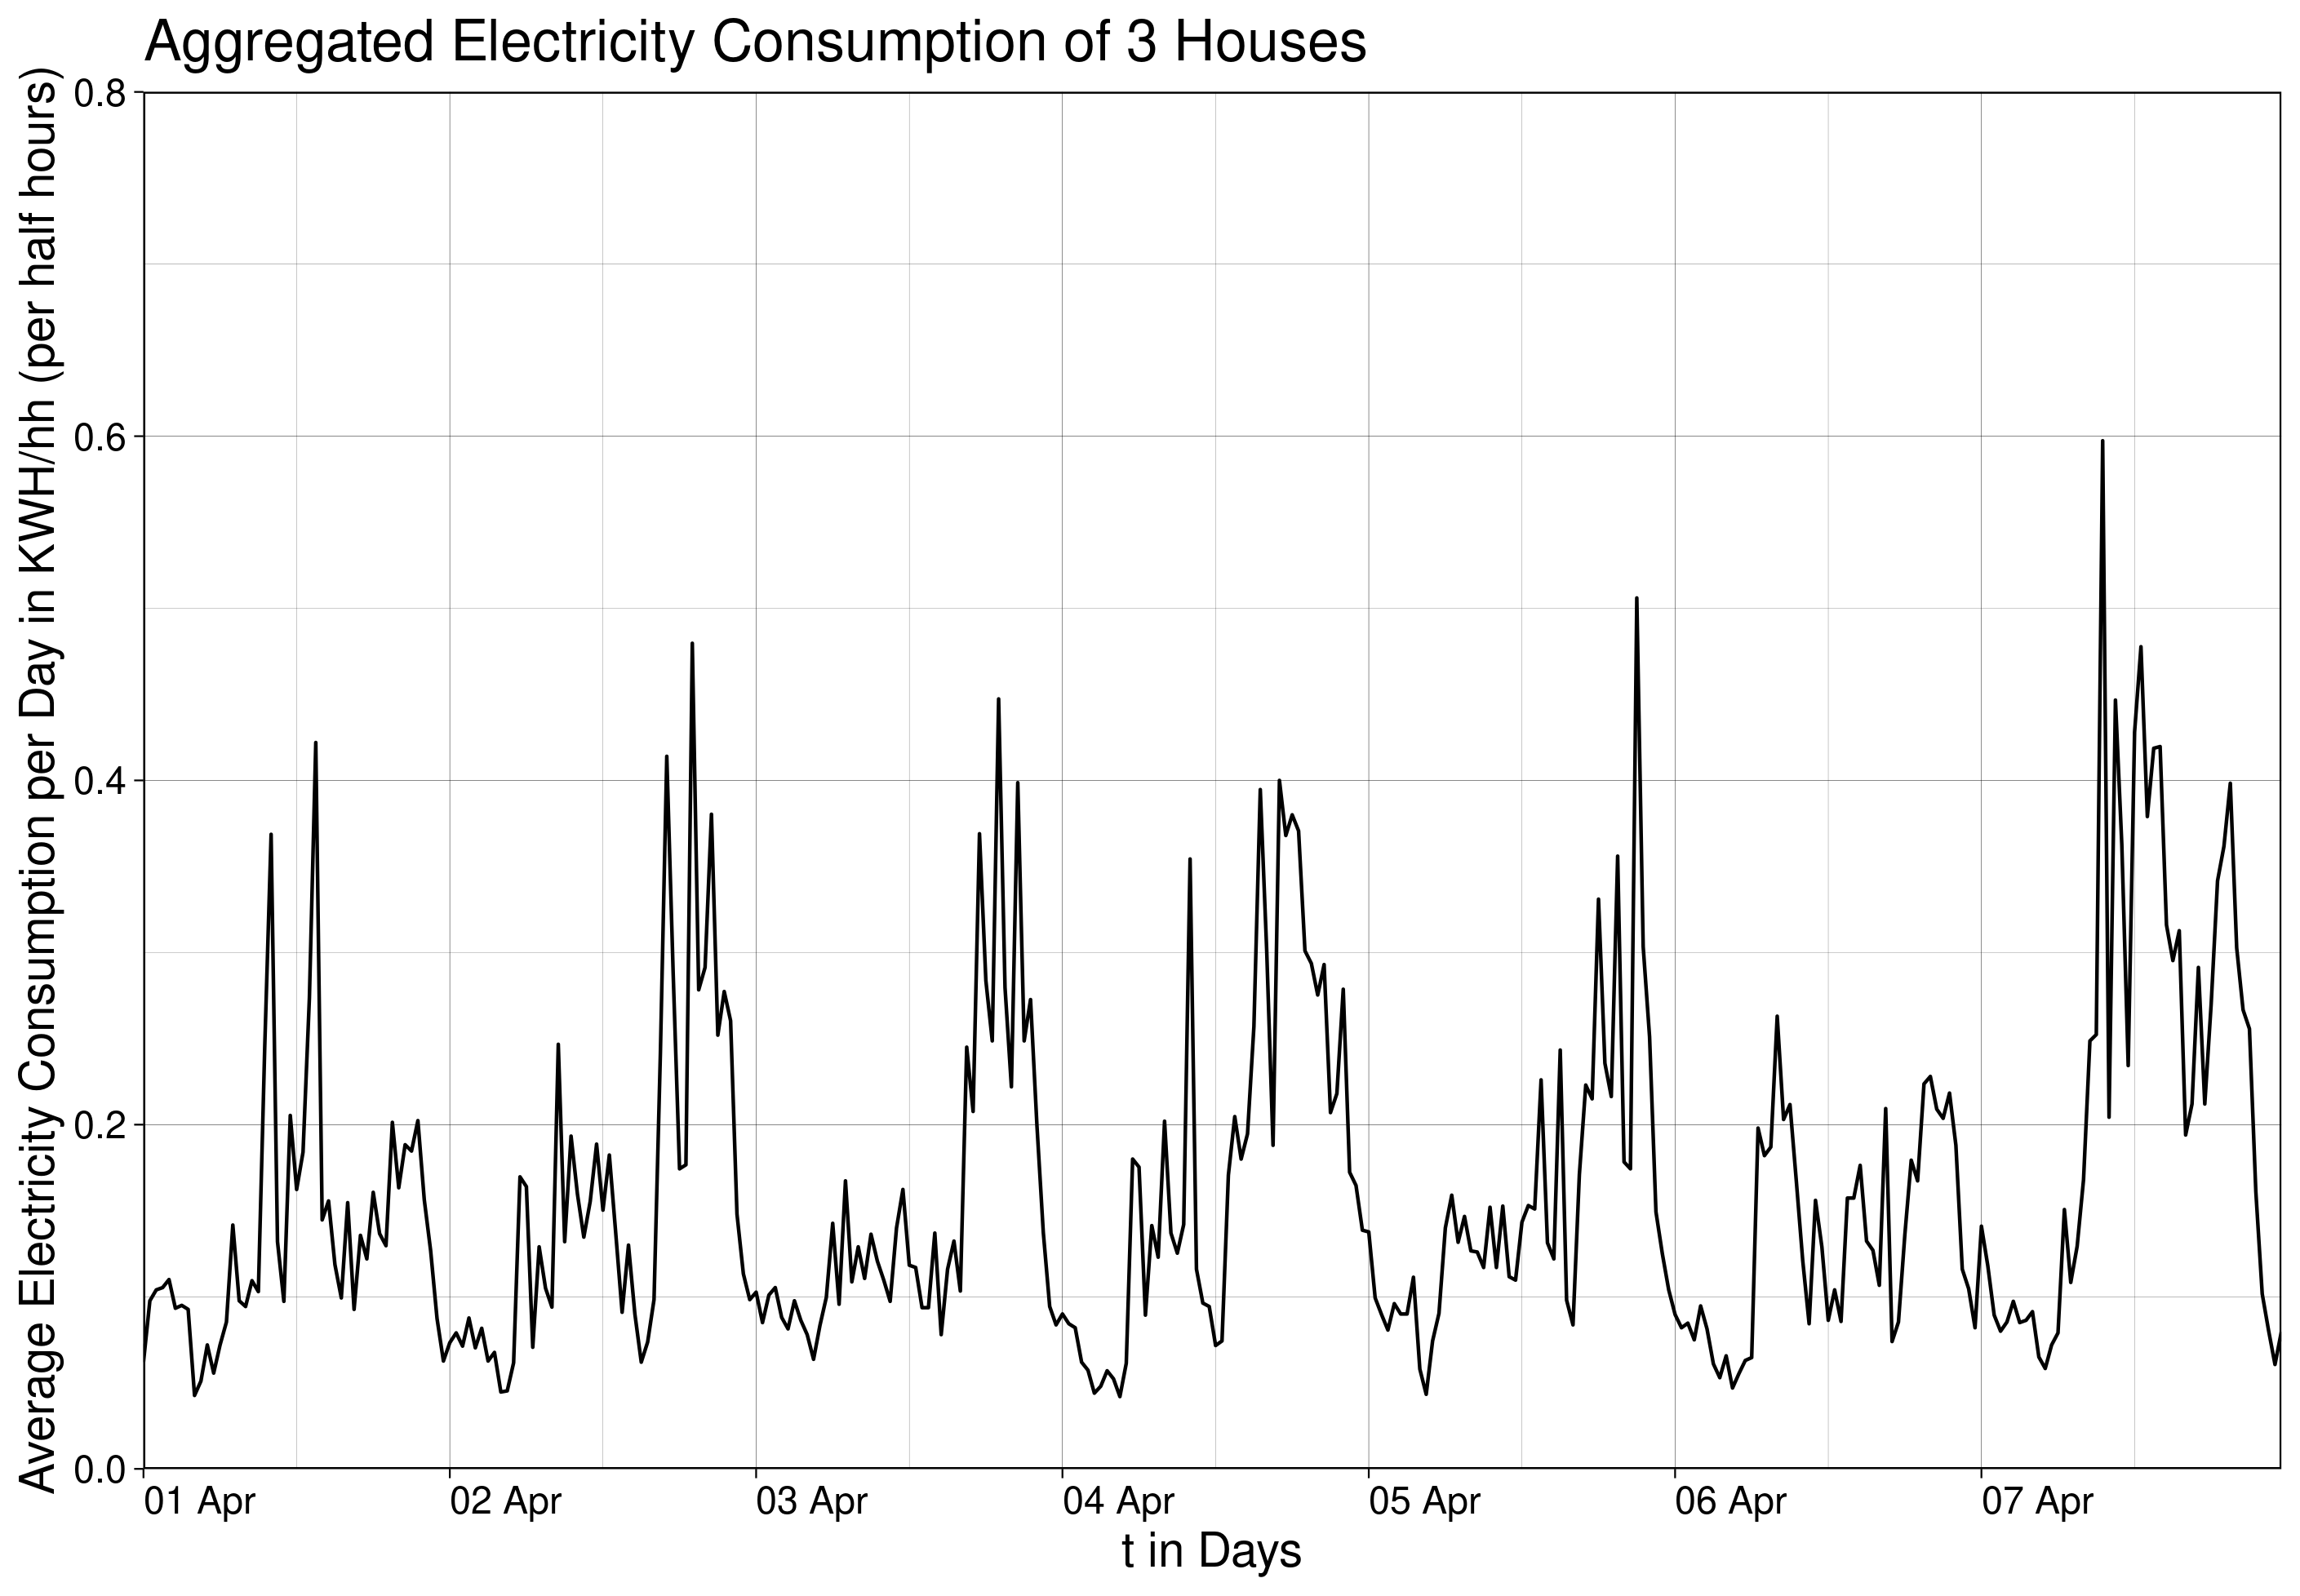
\includegraphics[width=0.8\columnwidth]{images/Aggregated Electricity Consumption of 3 Houses5.png}
\caption[Aggregated Electricity Consumption of 3 Houses of the 2nd Experiment]{}
\label{img:3_Houses_weekly}
\end{figure}

\nopagebreak
\afterpage{%
\begin{figure}[!p]
\centering
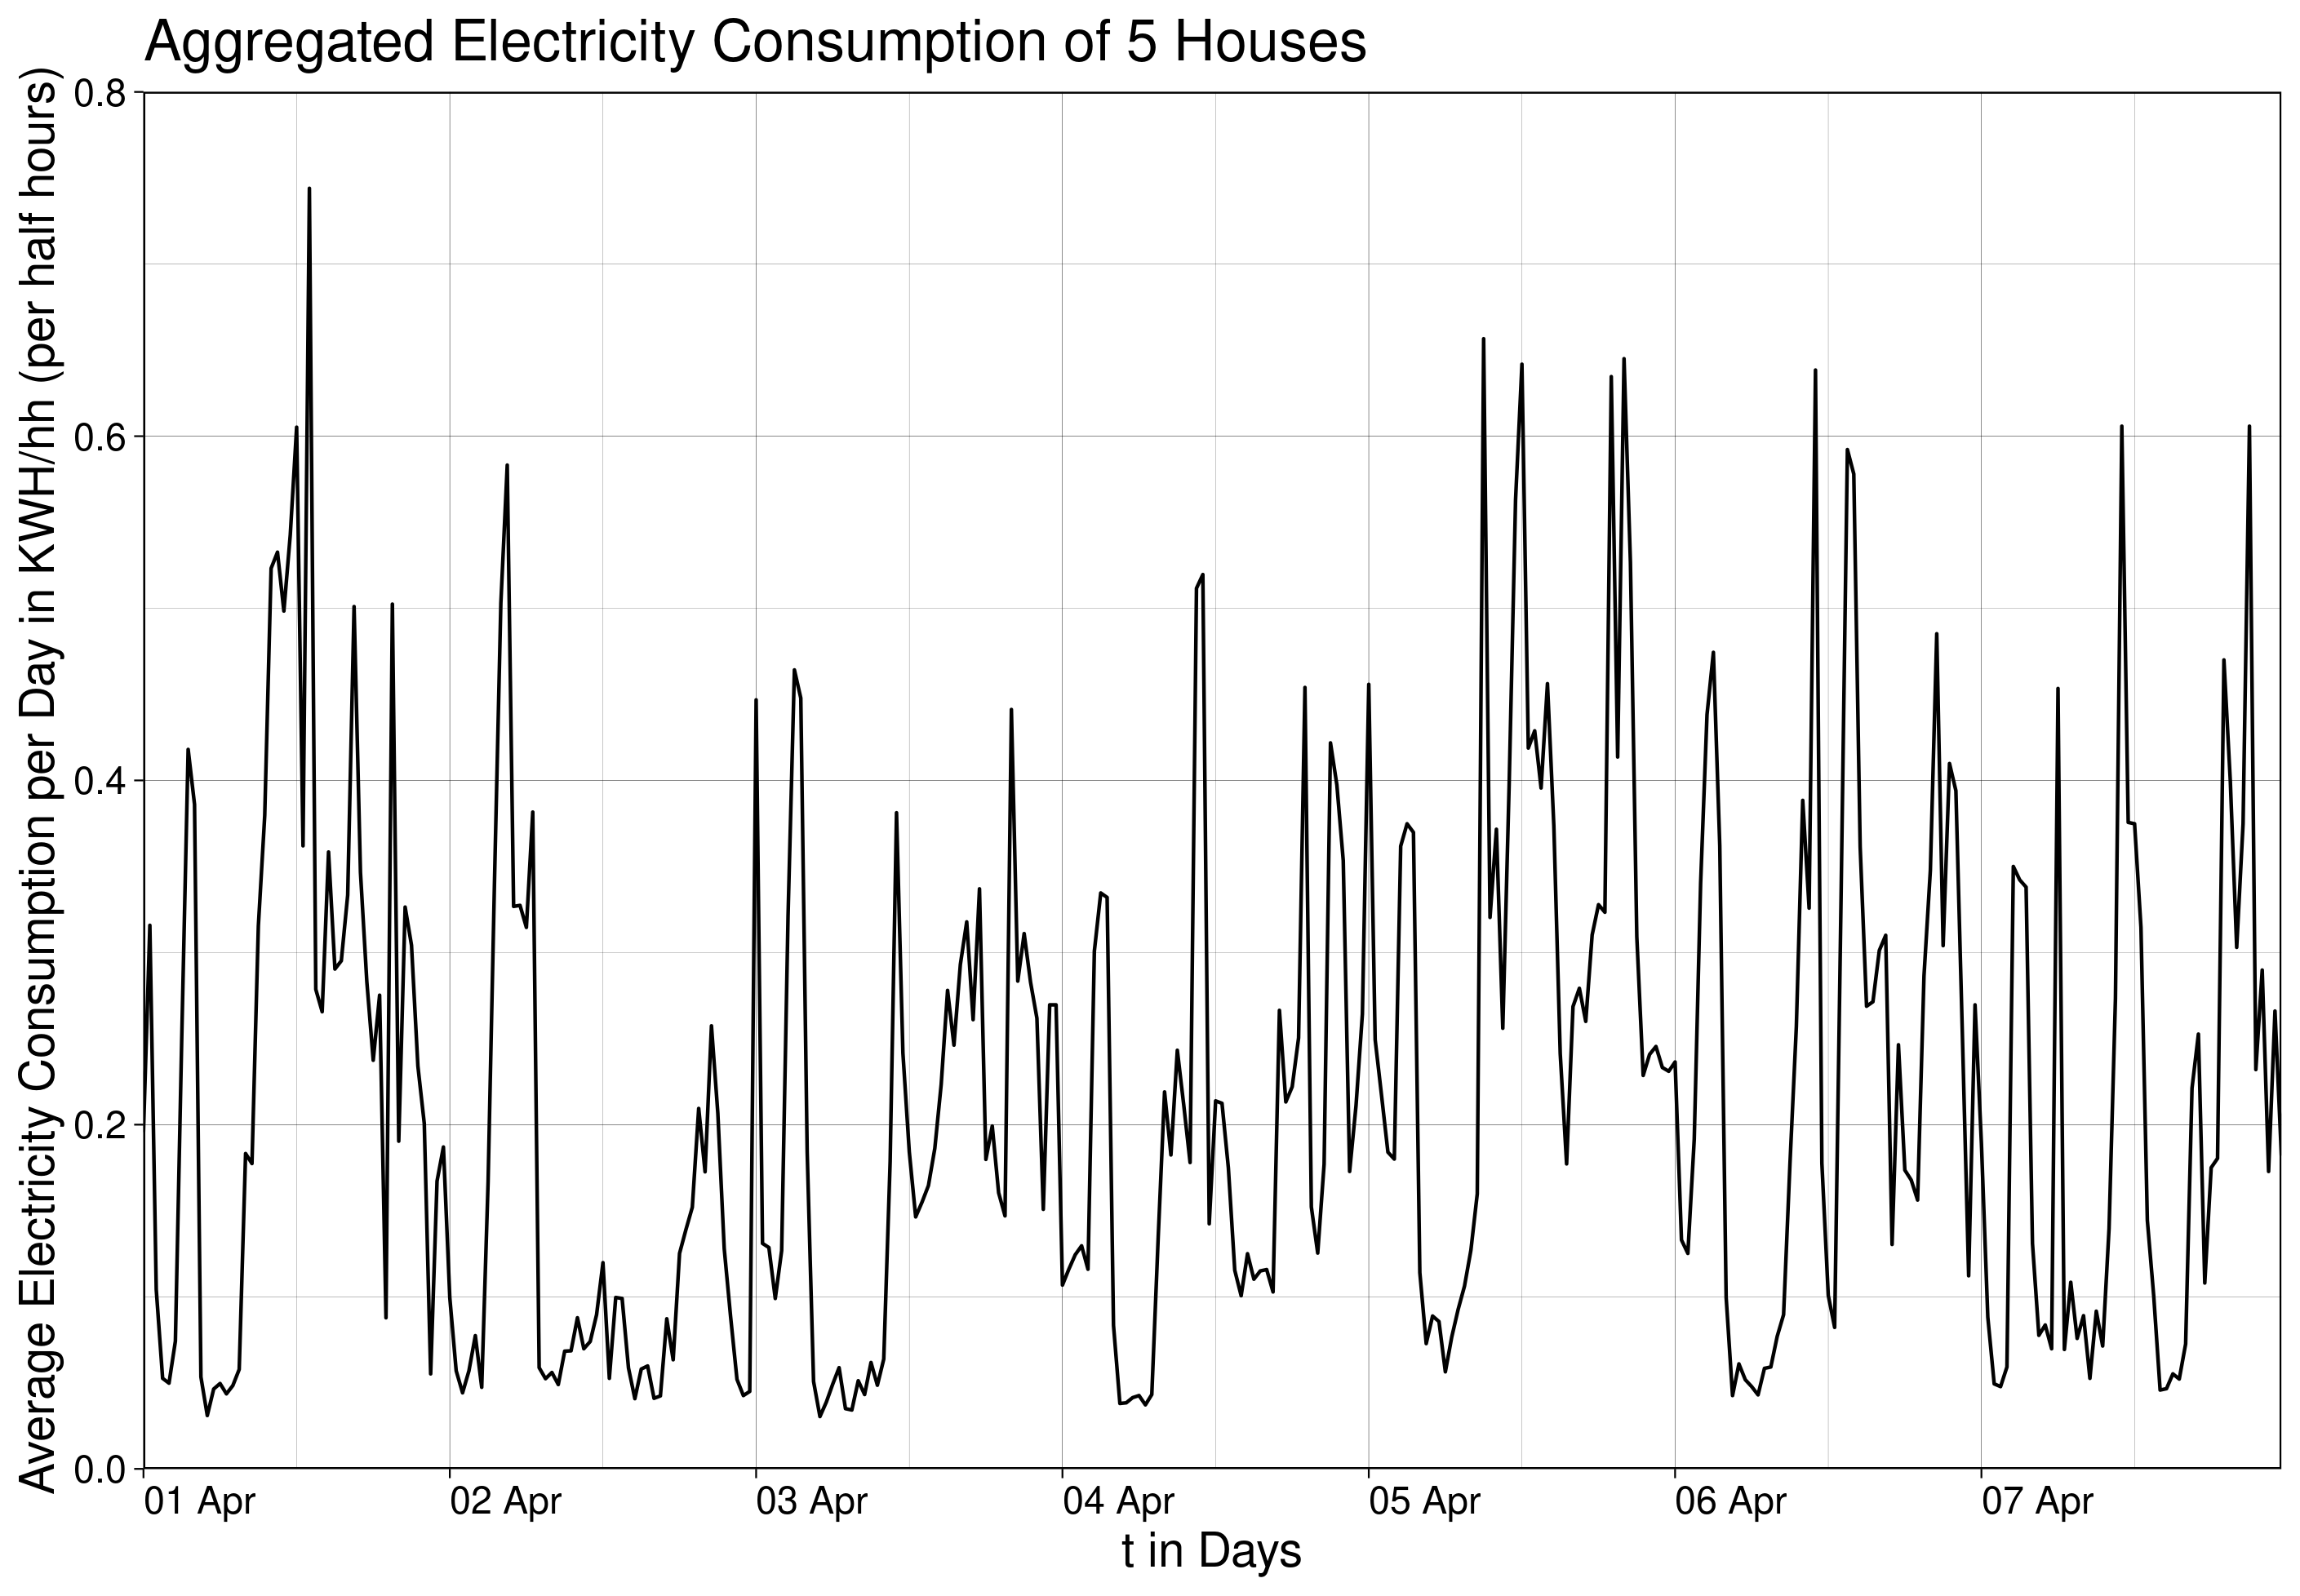
\includegraphics[width=0.85\textwidth]{images/Aggregated Electricity Consumption of 5 Houses5.png}
\caption[Aggregated Electricity Consumption of 5 Houses of the 2nd Experiment]{}
\label{img:5_Houses_weekly}
\end{figure}
\begin{figure}[!p]
\centering
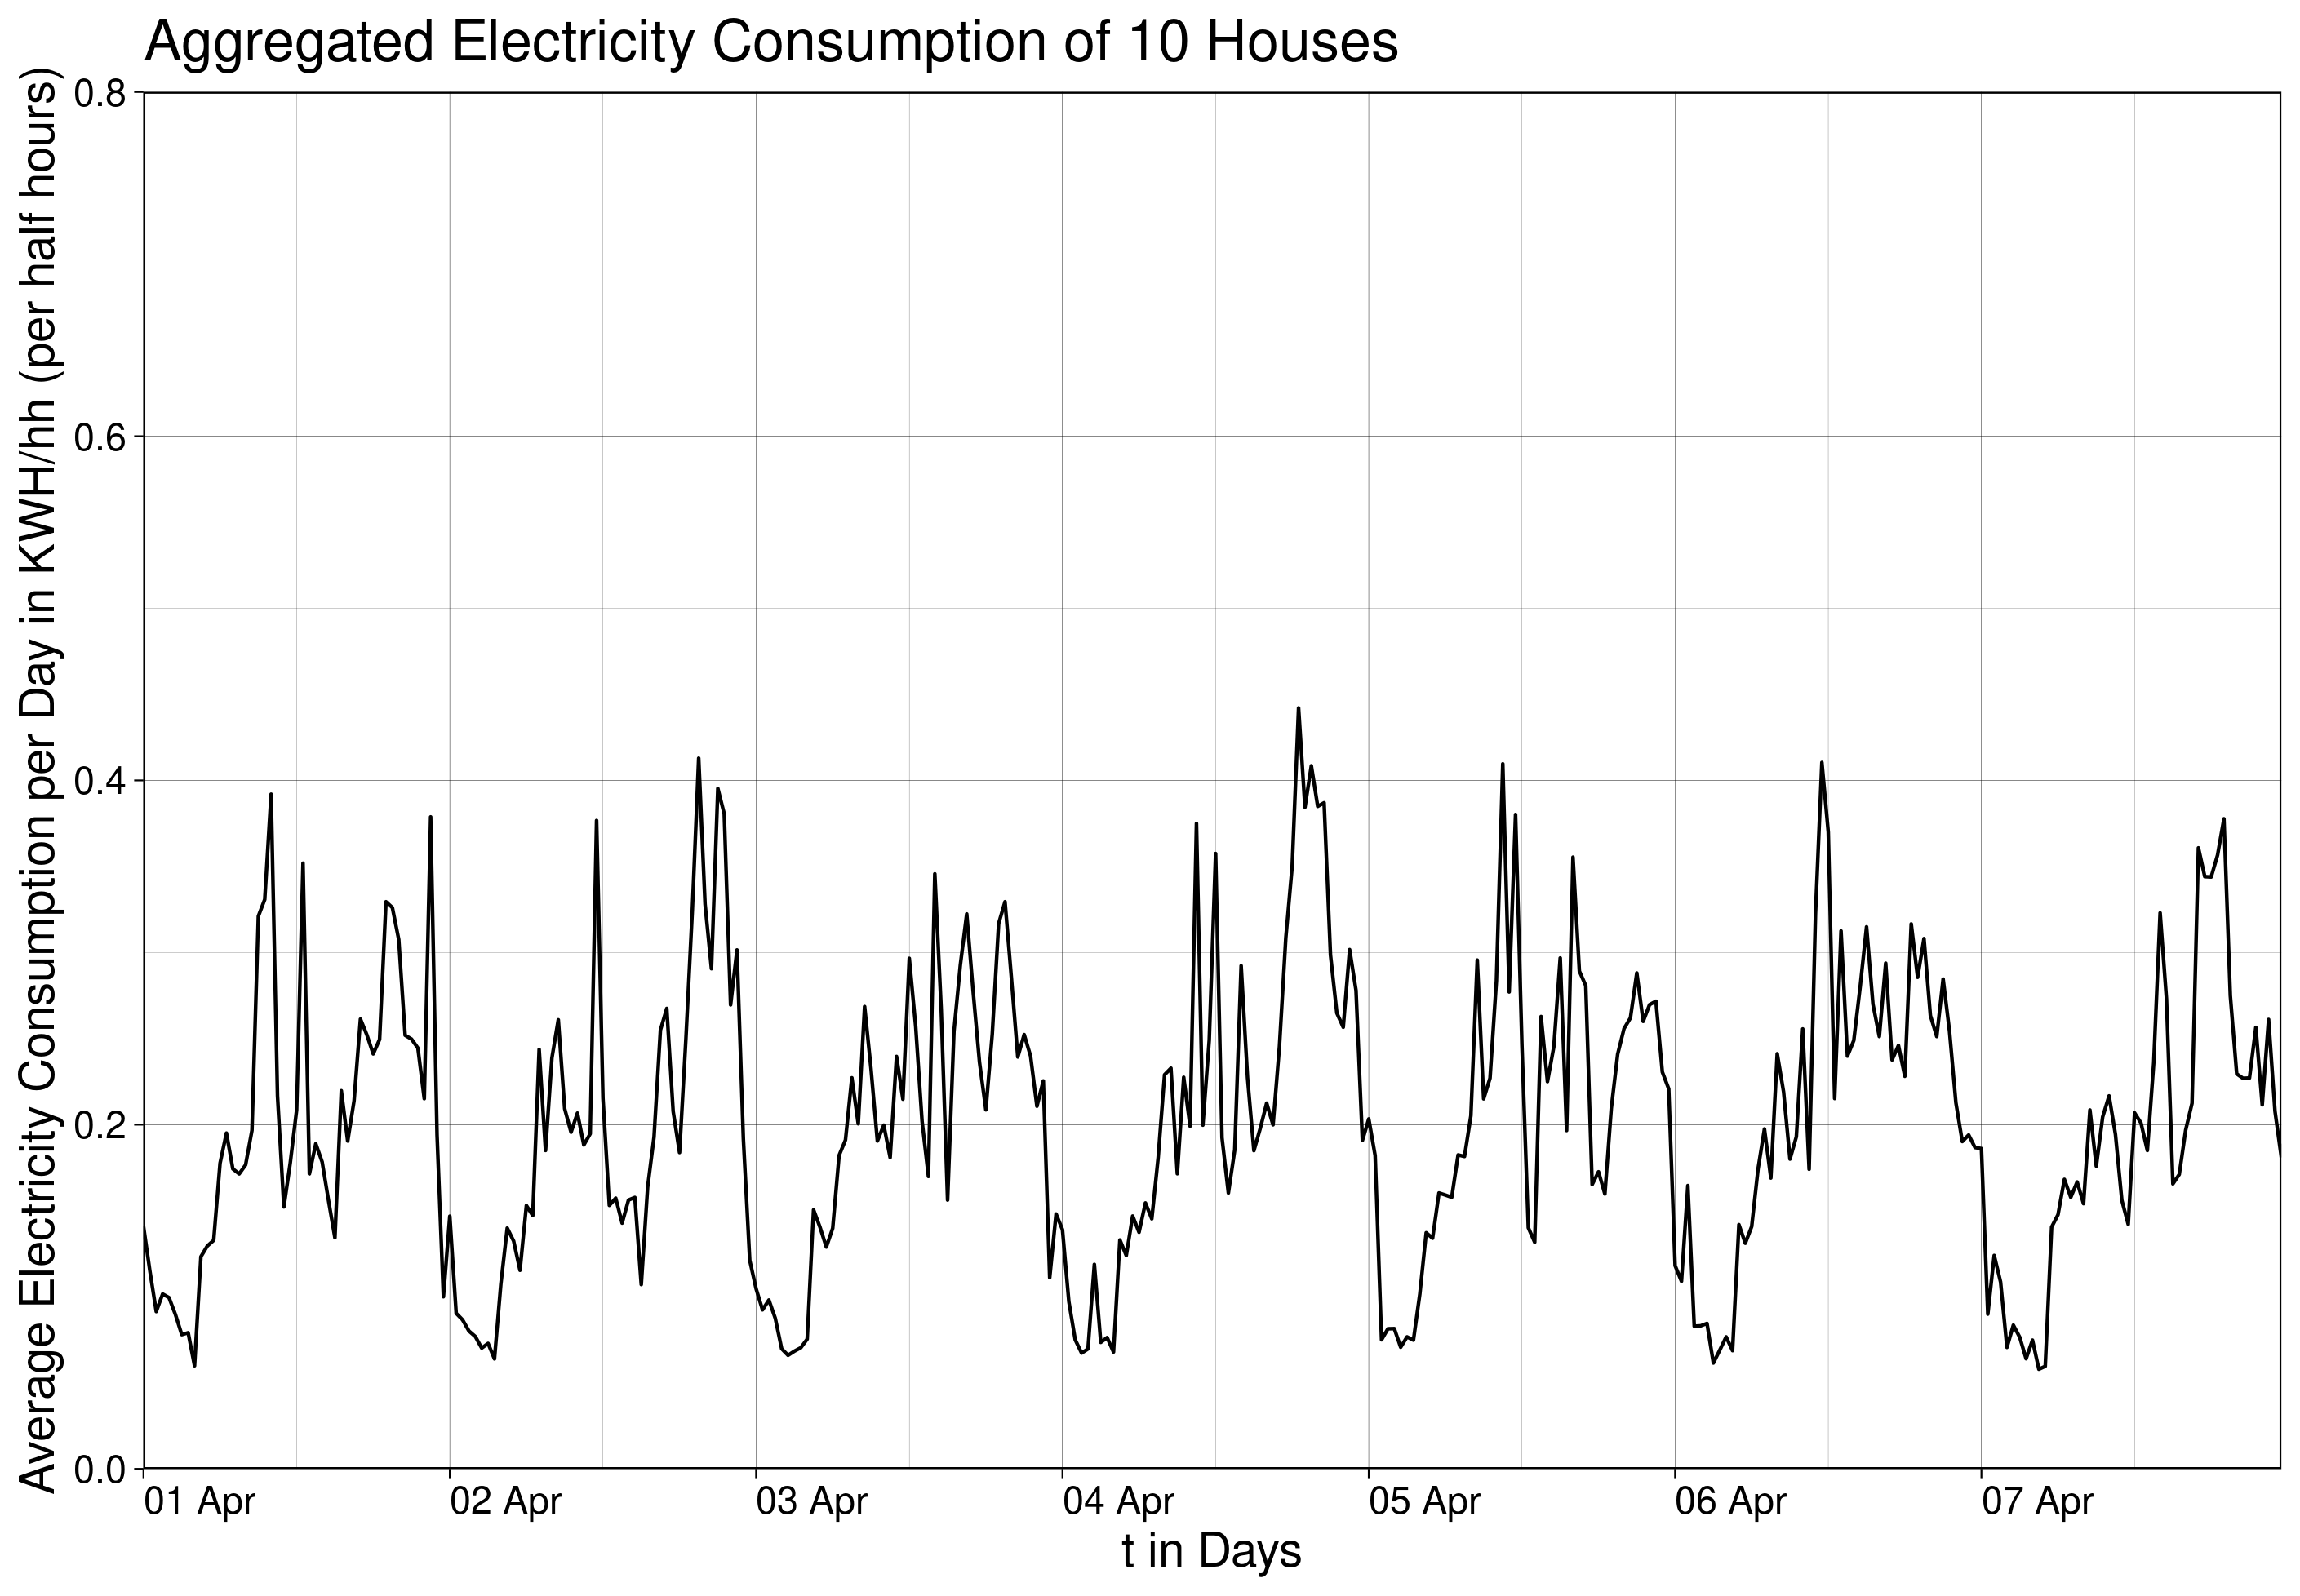
\includegraphics[width=0.85\textwidth]{images/Aggregated Electricity Consumption of 10 Houses5.png}
\caption[Aggregated Electricity Consumption of 10 Houses of the 2nd Experiment]{}
\label{img:10_Houses_weekly}
\end{figure}
\clearpage
}
\afterpage{%
\begin{figure}[!p]
\centering
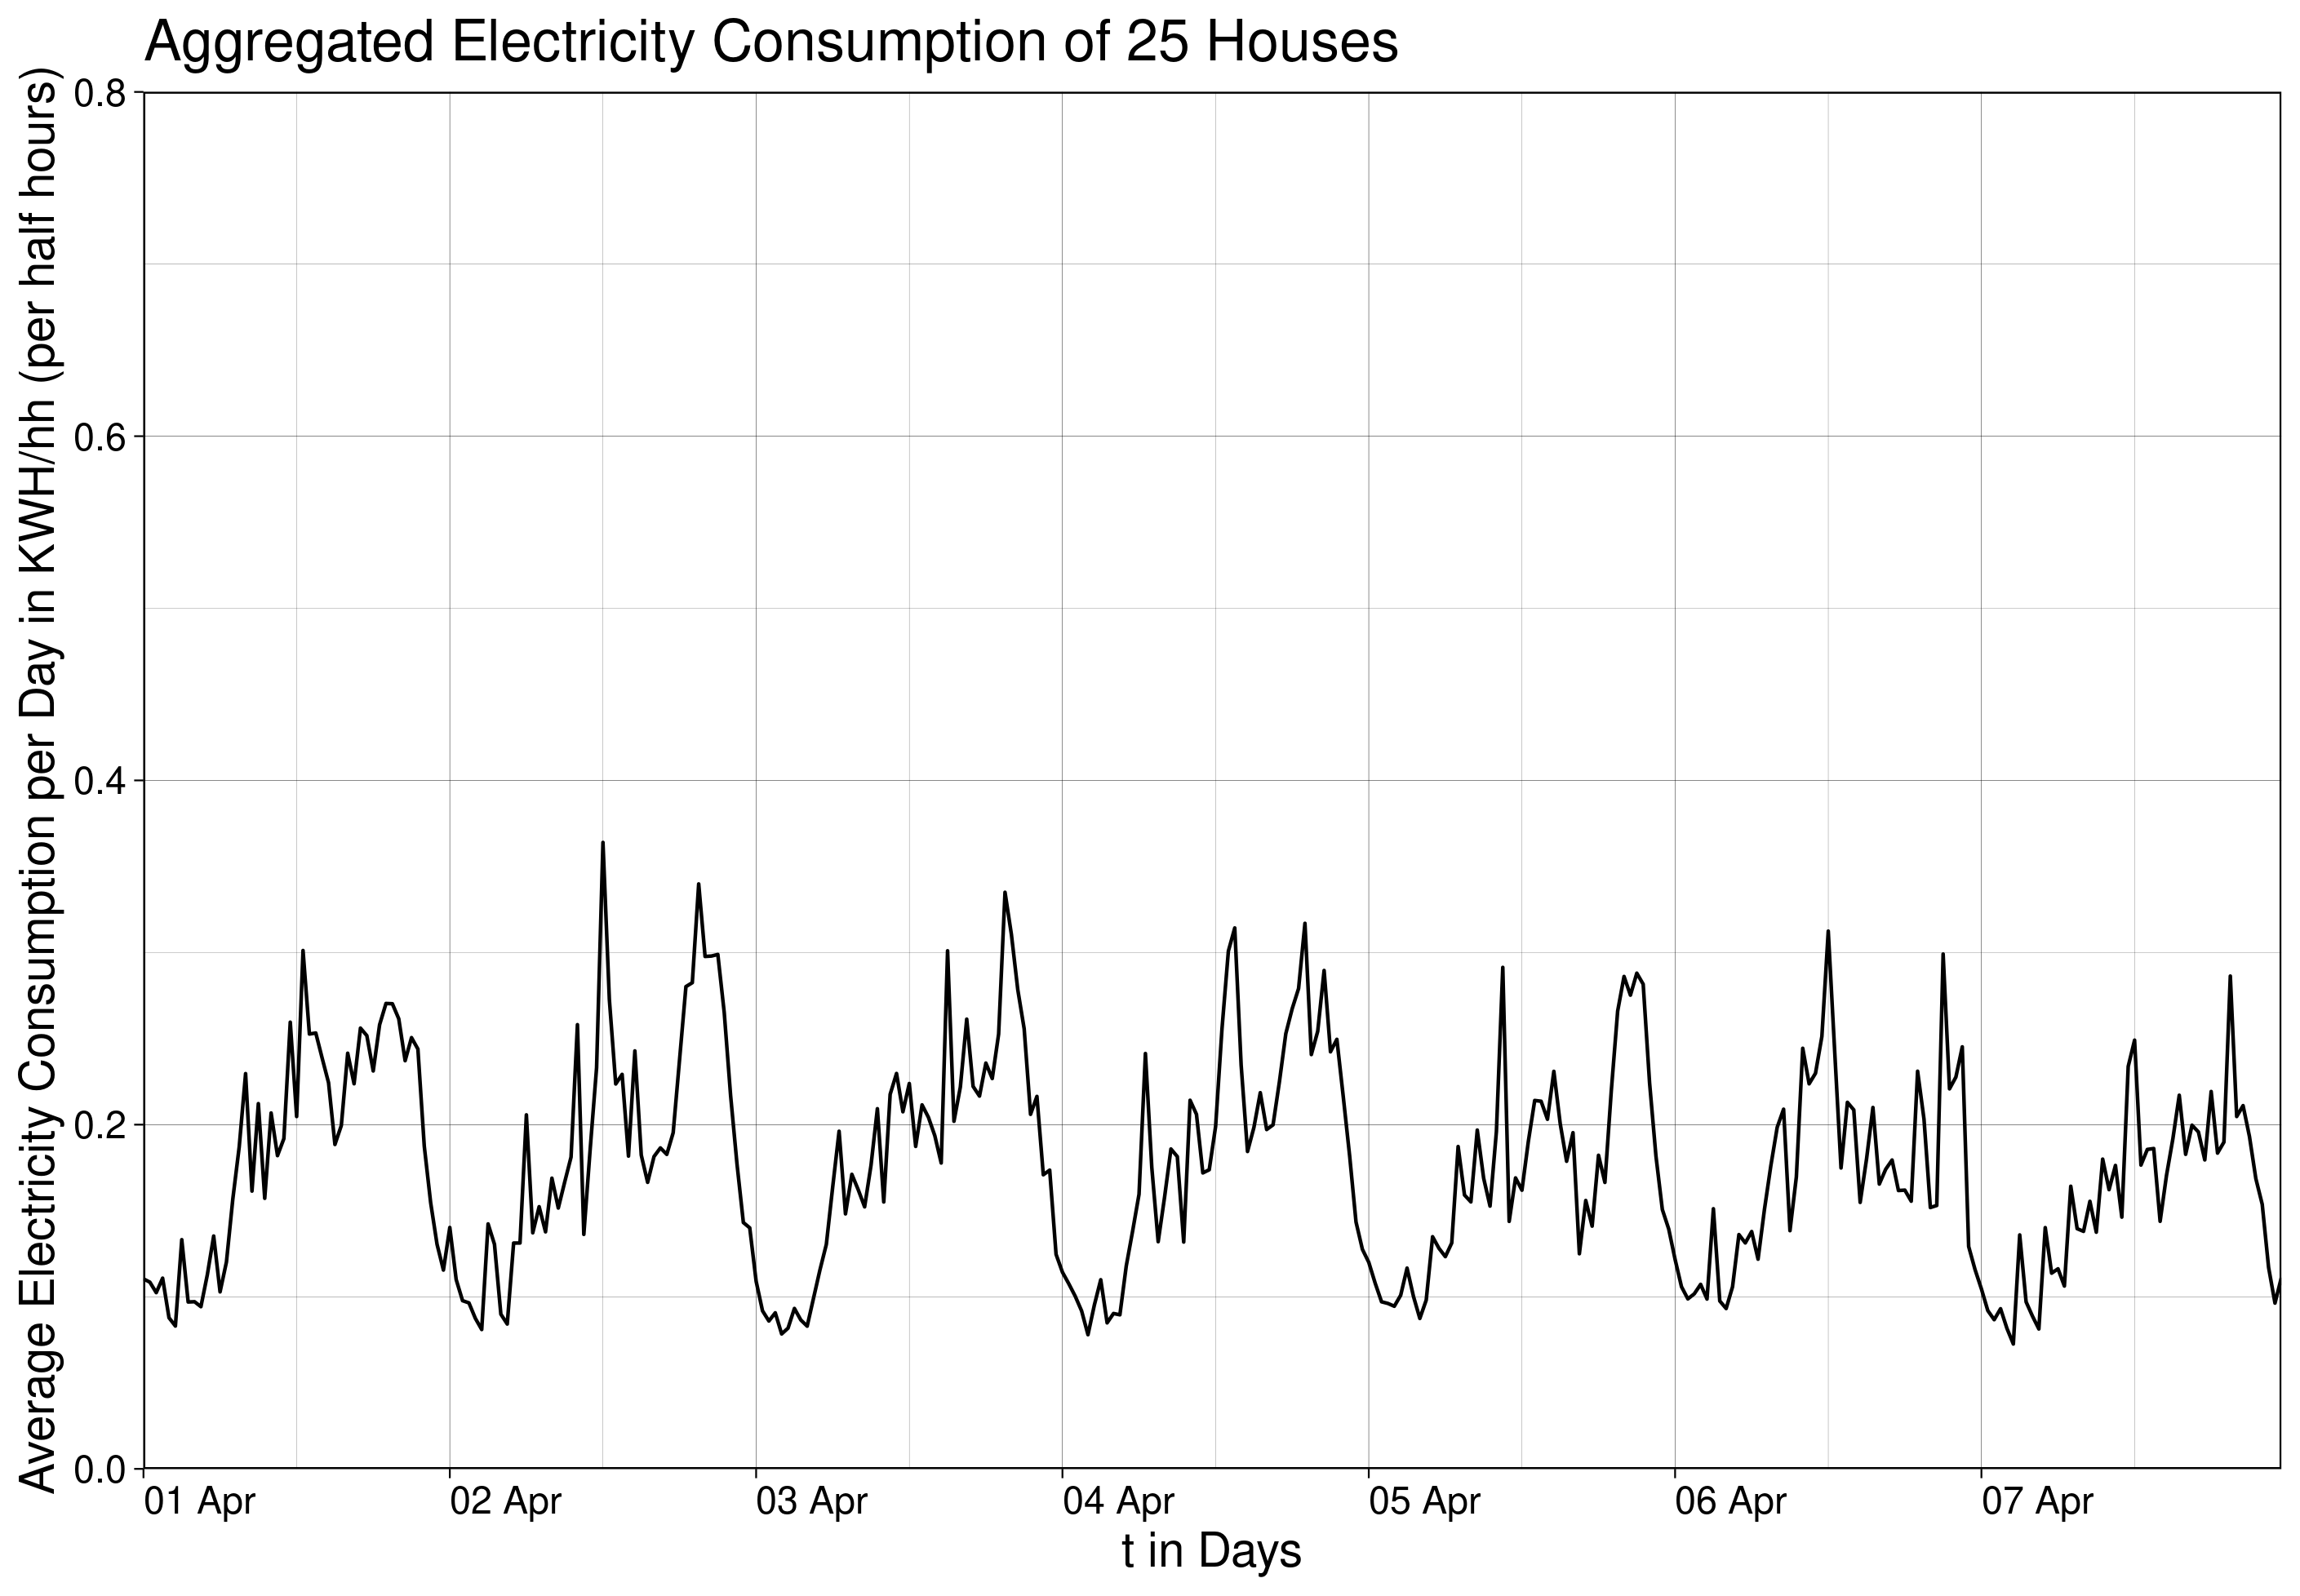
\includegraphics[width=0.85\textwidth]{images/Aggregated Electricity Consumption of 25 Houses5.png}
\caption[Aggregated Electricity Consumption of 25 Houses of the 2nd Experiment]{}
\label{img:25_Houses_weekly}
\end{figure}
\begin{figure}[!p]
\centering
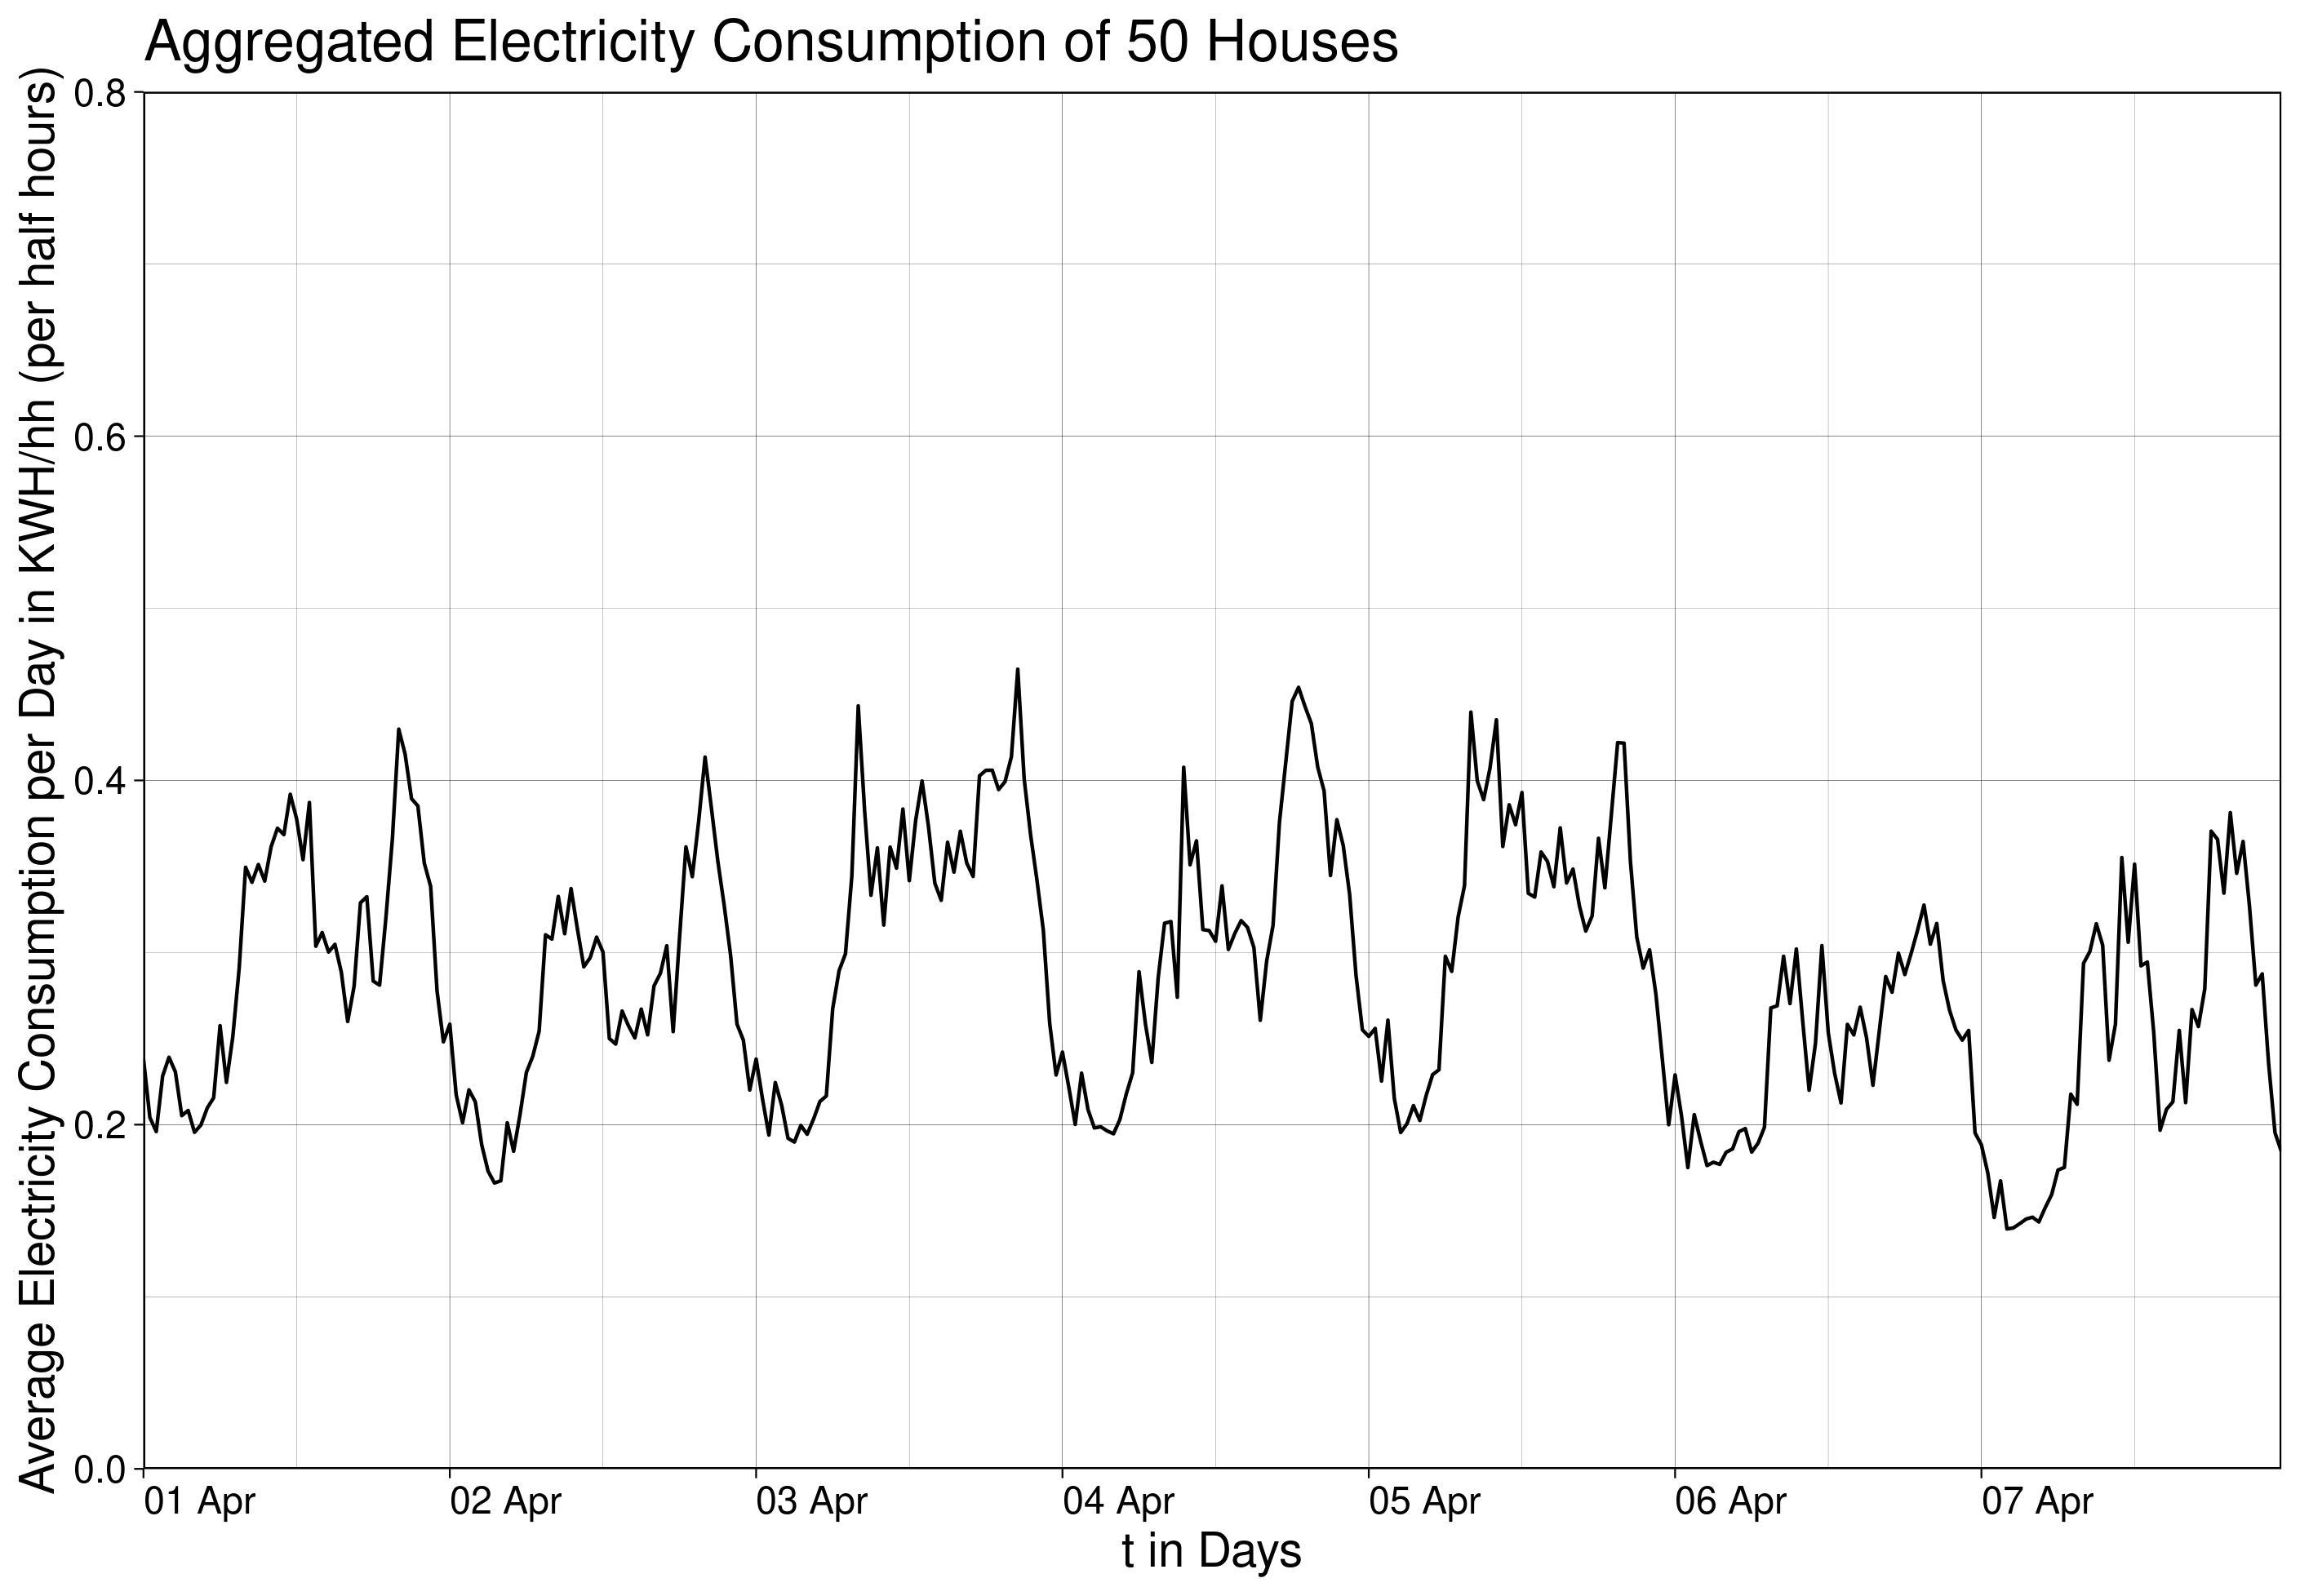
\includegraphics[width=0.85\textwidth]{images/Aggregated Electricity Consumption of 50 Houses5.png}
\caption[Aggregated Electricity Consumption of 50 Houses of the 2nd Experiment]{}
\label{img:50_Houses_weekly}
\end{figure}
\clearpage
}
\afterpage{%
\begin{figure}[!p]
\centering
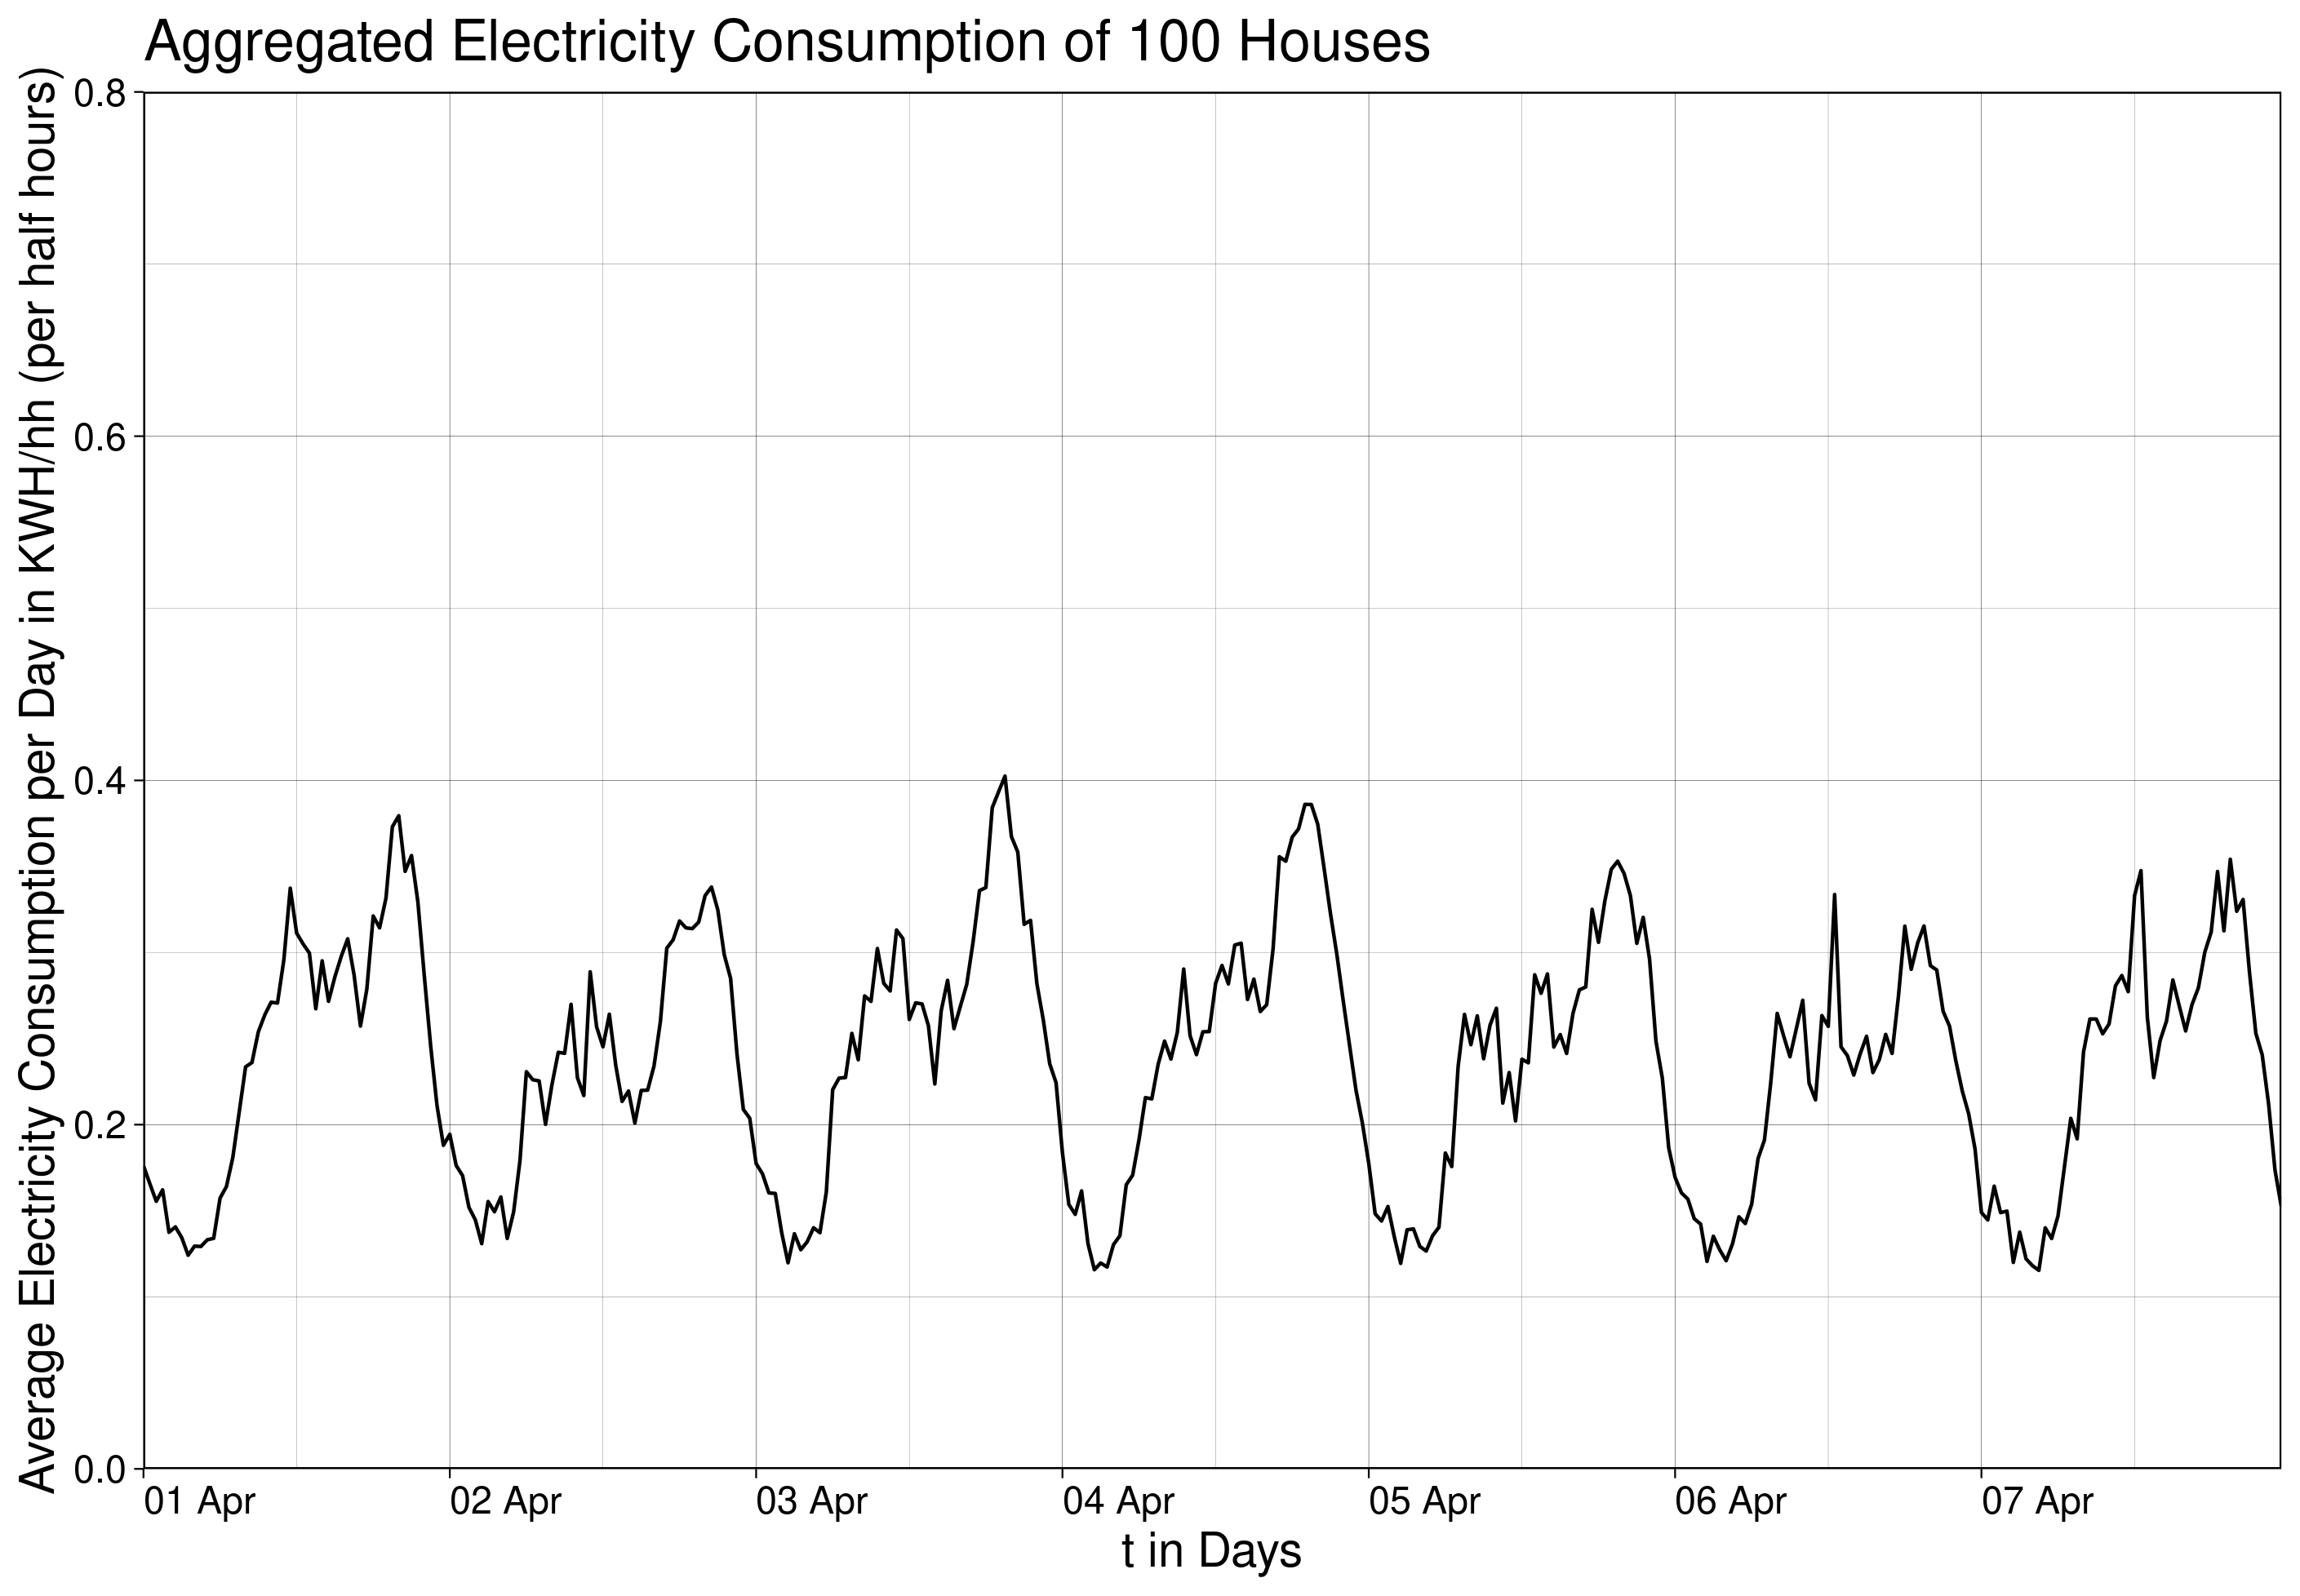
\includegraphics[width=0.85\textwidth]{images/Aggregated Electricity Consumption of 100 Houses5.png}
\caption[Aggregated Electricity Consumption of 100 Houses of the 2nd Experiment]{}
\label{img:100_Houses_weekly}
\end{figure}
\begin{figure}[!p]
\centering
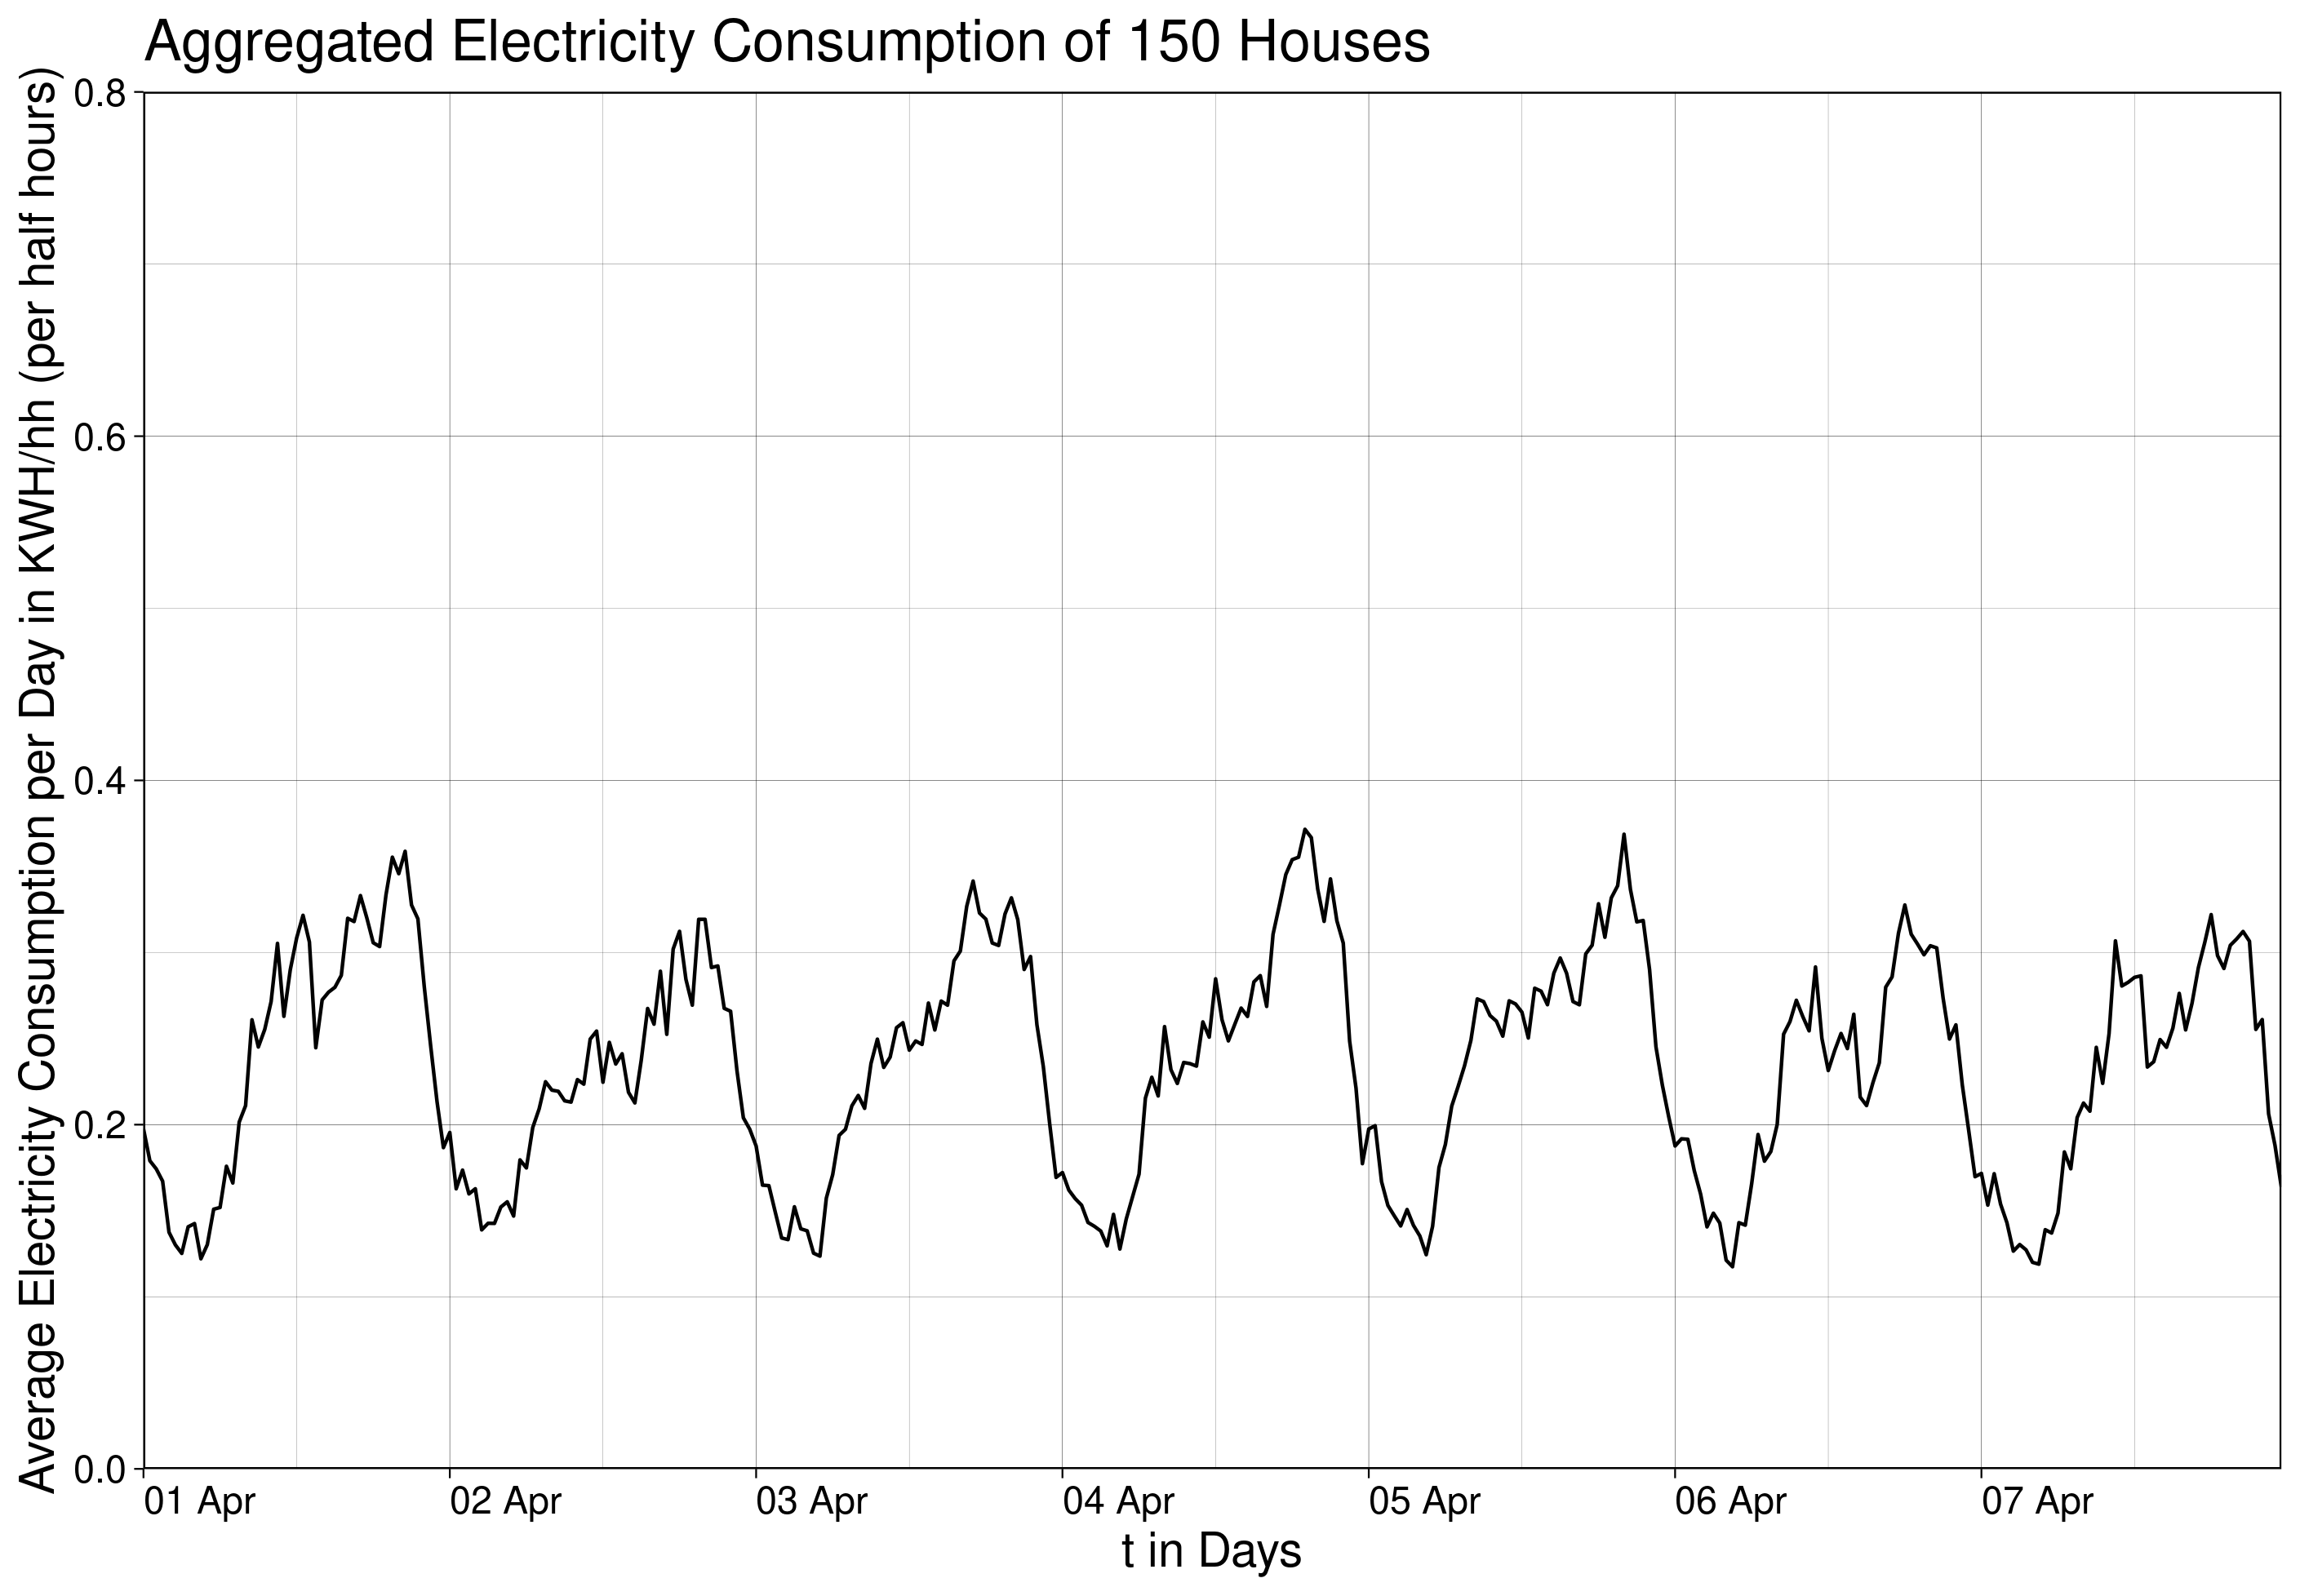
\includegraphics[width=0.85\textwidth]{images/Aggregated Electricity Consumption of 150 Houses5.png}
\caption[Aggregated Electricity Consumption of 150 Houses of the 2nd Experiment]{}
\label{img:150_houses_weekly}
\end{figure}
\clearpage
}
\afterpage{%
\begin{figure}[!p]
\centering
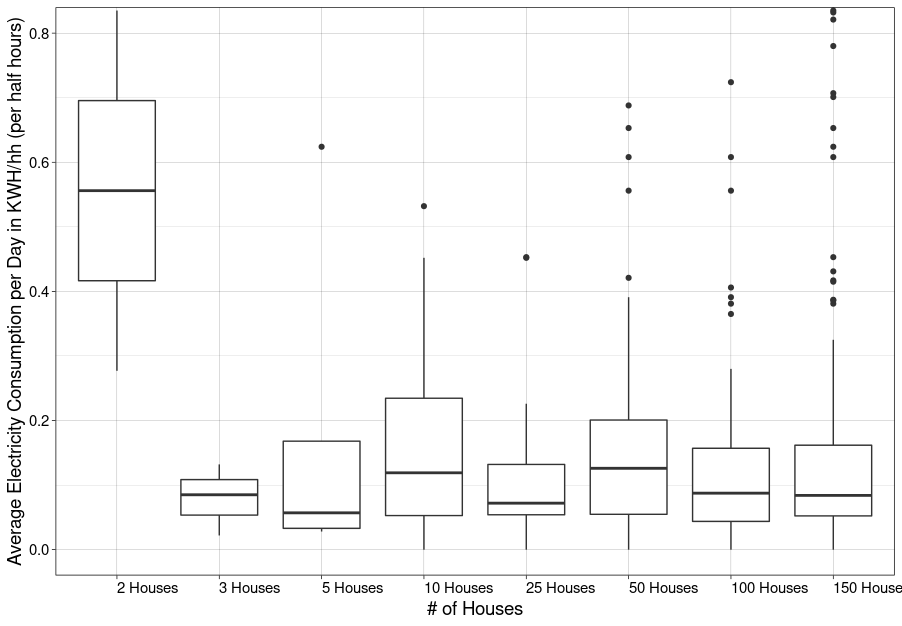
\includegraphics[width=0.85\textwidth]{images/Boxplot_test4.png}
\caption[Boxplot of the first Week]{Boxplot of the average electricity consumption in the first week of the experiment.}
\label{img:boxplot_first}
\end{figure}
\begin{figure}[!p]
\centering
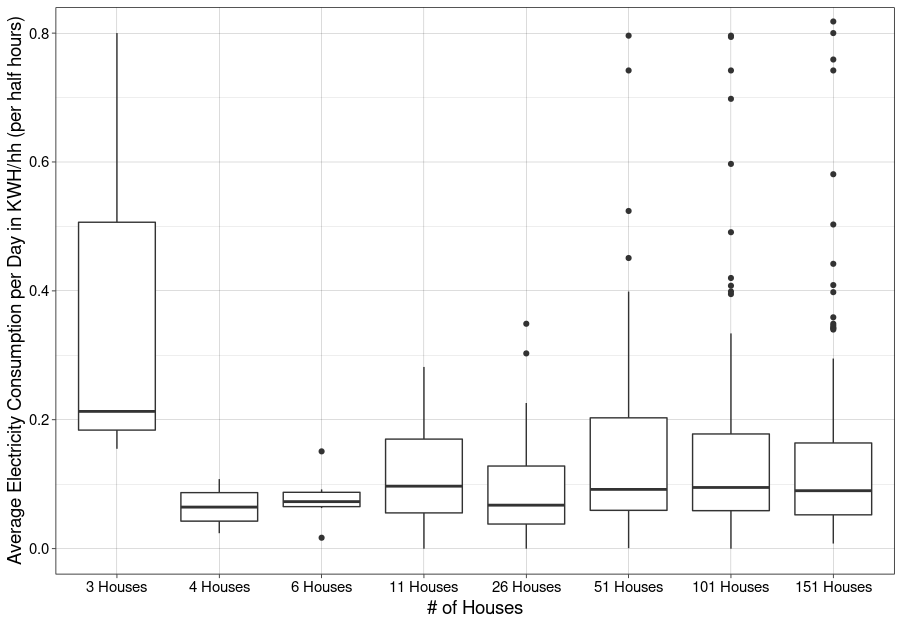
\includegraphics[width=0.85\textwidth]{images/boxplot_2nd_week.png}
\caption[Boxplot of the second Week]{Boxplot of the average electricity consumption in the second week of the experiment.}
\label{img:boxplot_second}
\end{figure}
\clearpage
}

\afterpage{%
\begin{figure}[!p]
\centering
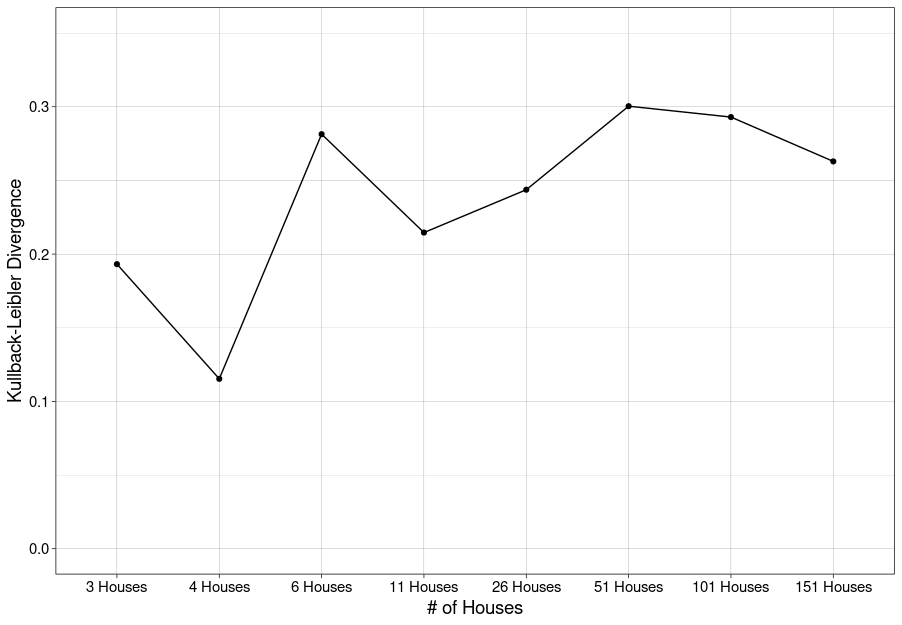
\includegraphics[width=0.85\textwidth]{images/KLD_Test2.png}
\caption[Kullback Leibler Divergence]{Kullback Leibler Divergence of the second week.}
\label{img:KLD}
\end{figure}
\begin{figure}[!p]
\centering
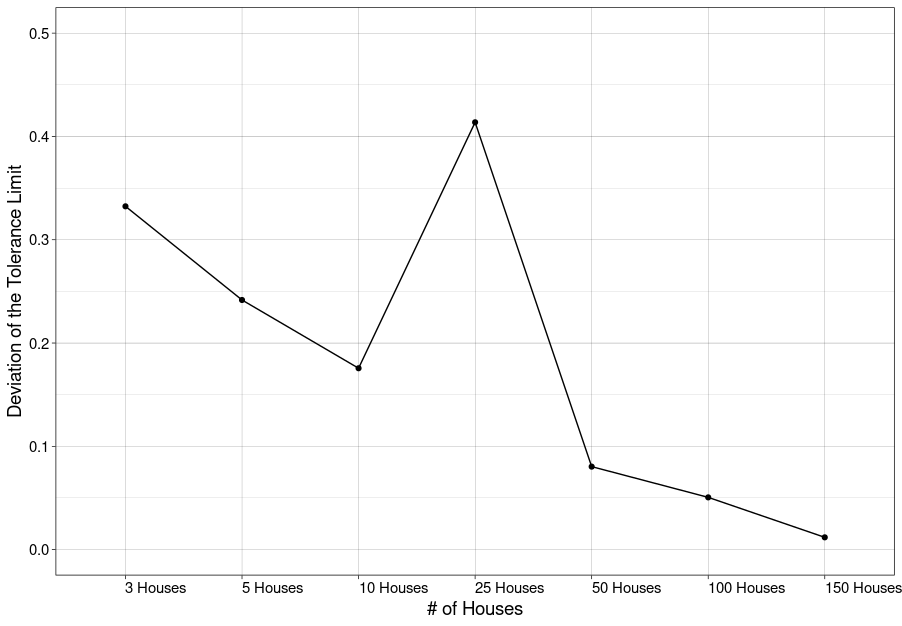
\includegraphics[width=0.85\textwidth]{images/Deviation1.png}
\caption[Deviation of the 2nd Experiment]{Deviation from the Tolerance Limit in the first week.}
\label{img:Dev_2nd}
\end{figure}
\clearpage
}
\afterpage{%
\begin{figure}[!p]
\centering
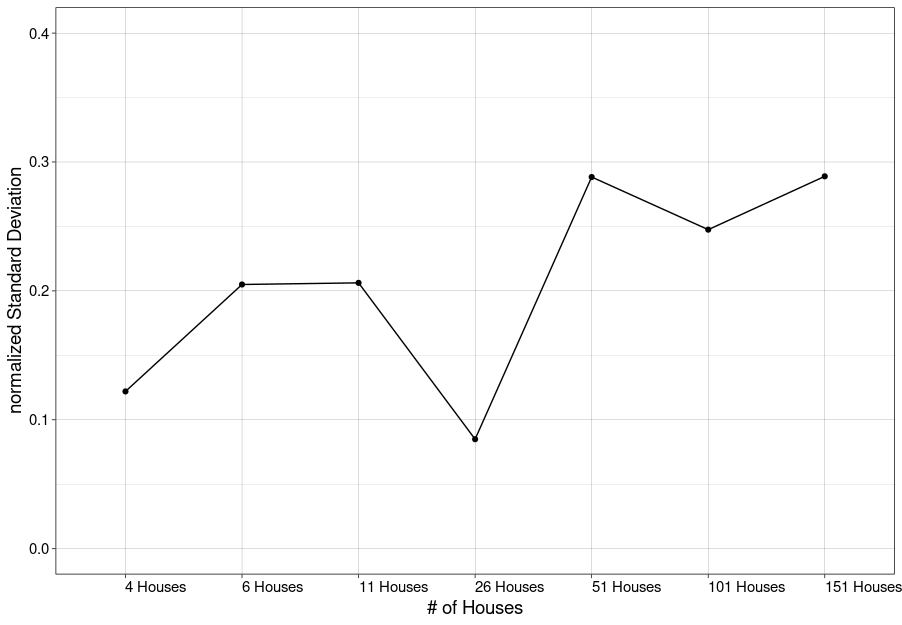
\includegraphics[width=0.85\textwidth]{images/standard_deviation2_test4.png}
\caption[Normalized Standard Deviation]{Normalized Standard Deviation of the second week.}
\label{img:SD}
\end{figure}
\clearpage
}

\chapter{Yearlong Experiments}
\enlargethispage{10}
\vspace*{-10\baseline}
\begin{figure}[H]
\centering
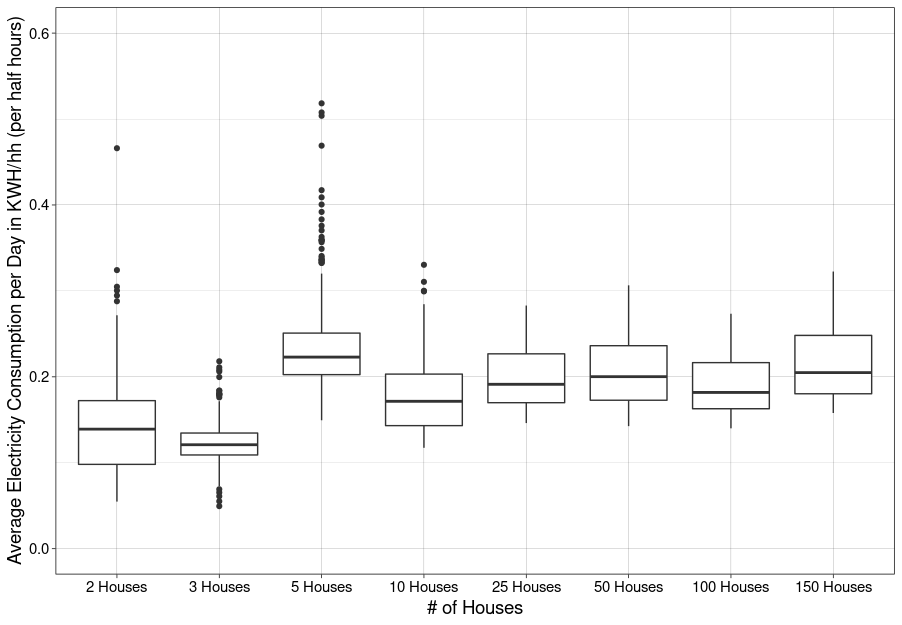
\includegraphics[width=0.8\columnwidth]{images/boxplot_neu_neu.png}
\caption[Boxplots of the Average Base Load]{Boxplots of the average electricity consumption.}
\label{img:Box}
\centering
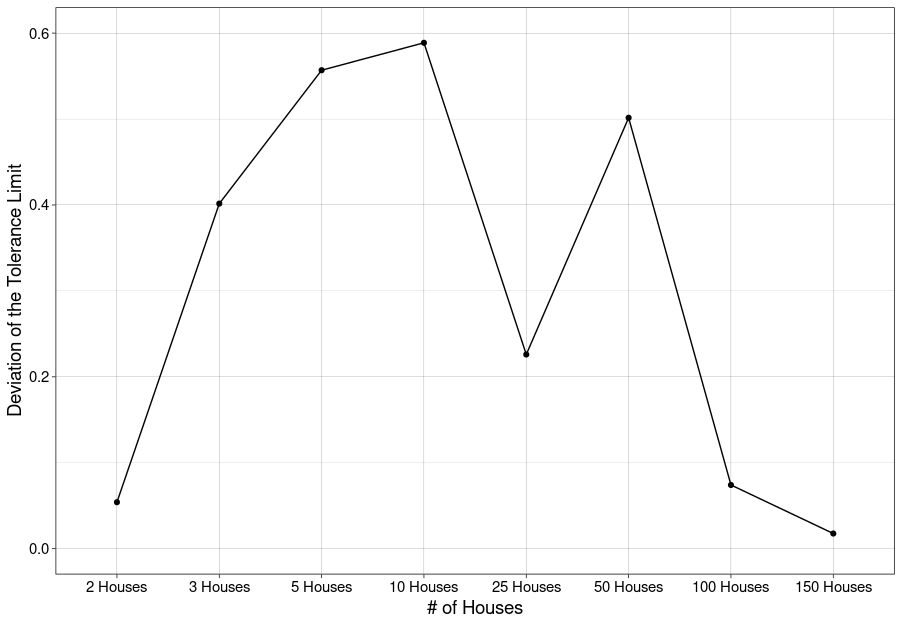
\includegraphics[width=0.8\columnwidth]{images/Deviation_Houses.png}
\caption[Deviation of the Standard Variance]{Deviation from the Tolerance Limit}
\label{img:Deviation}
\end{figure}
\nopagebreak
%Nachschauen mit den ferien im april bei 2 häusern
%durchschnittliche Mittelwert(von boxplots)
%ergebnisse der abweichung
%versuche wurden 2 mal wiederholt.
\afterpage{%
\begin{figure}[!p]
\centering
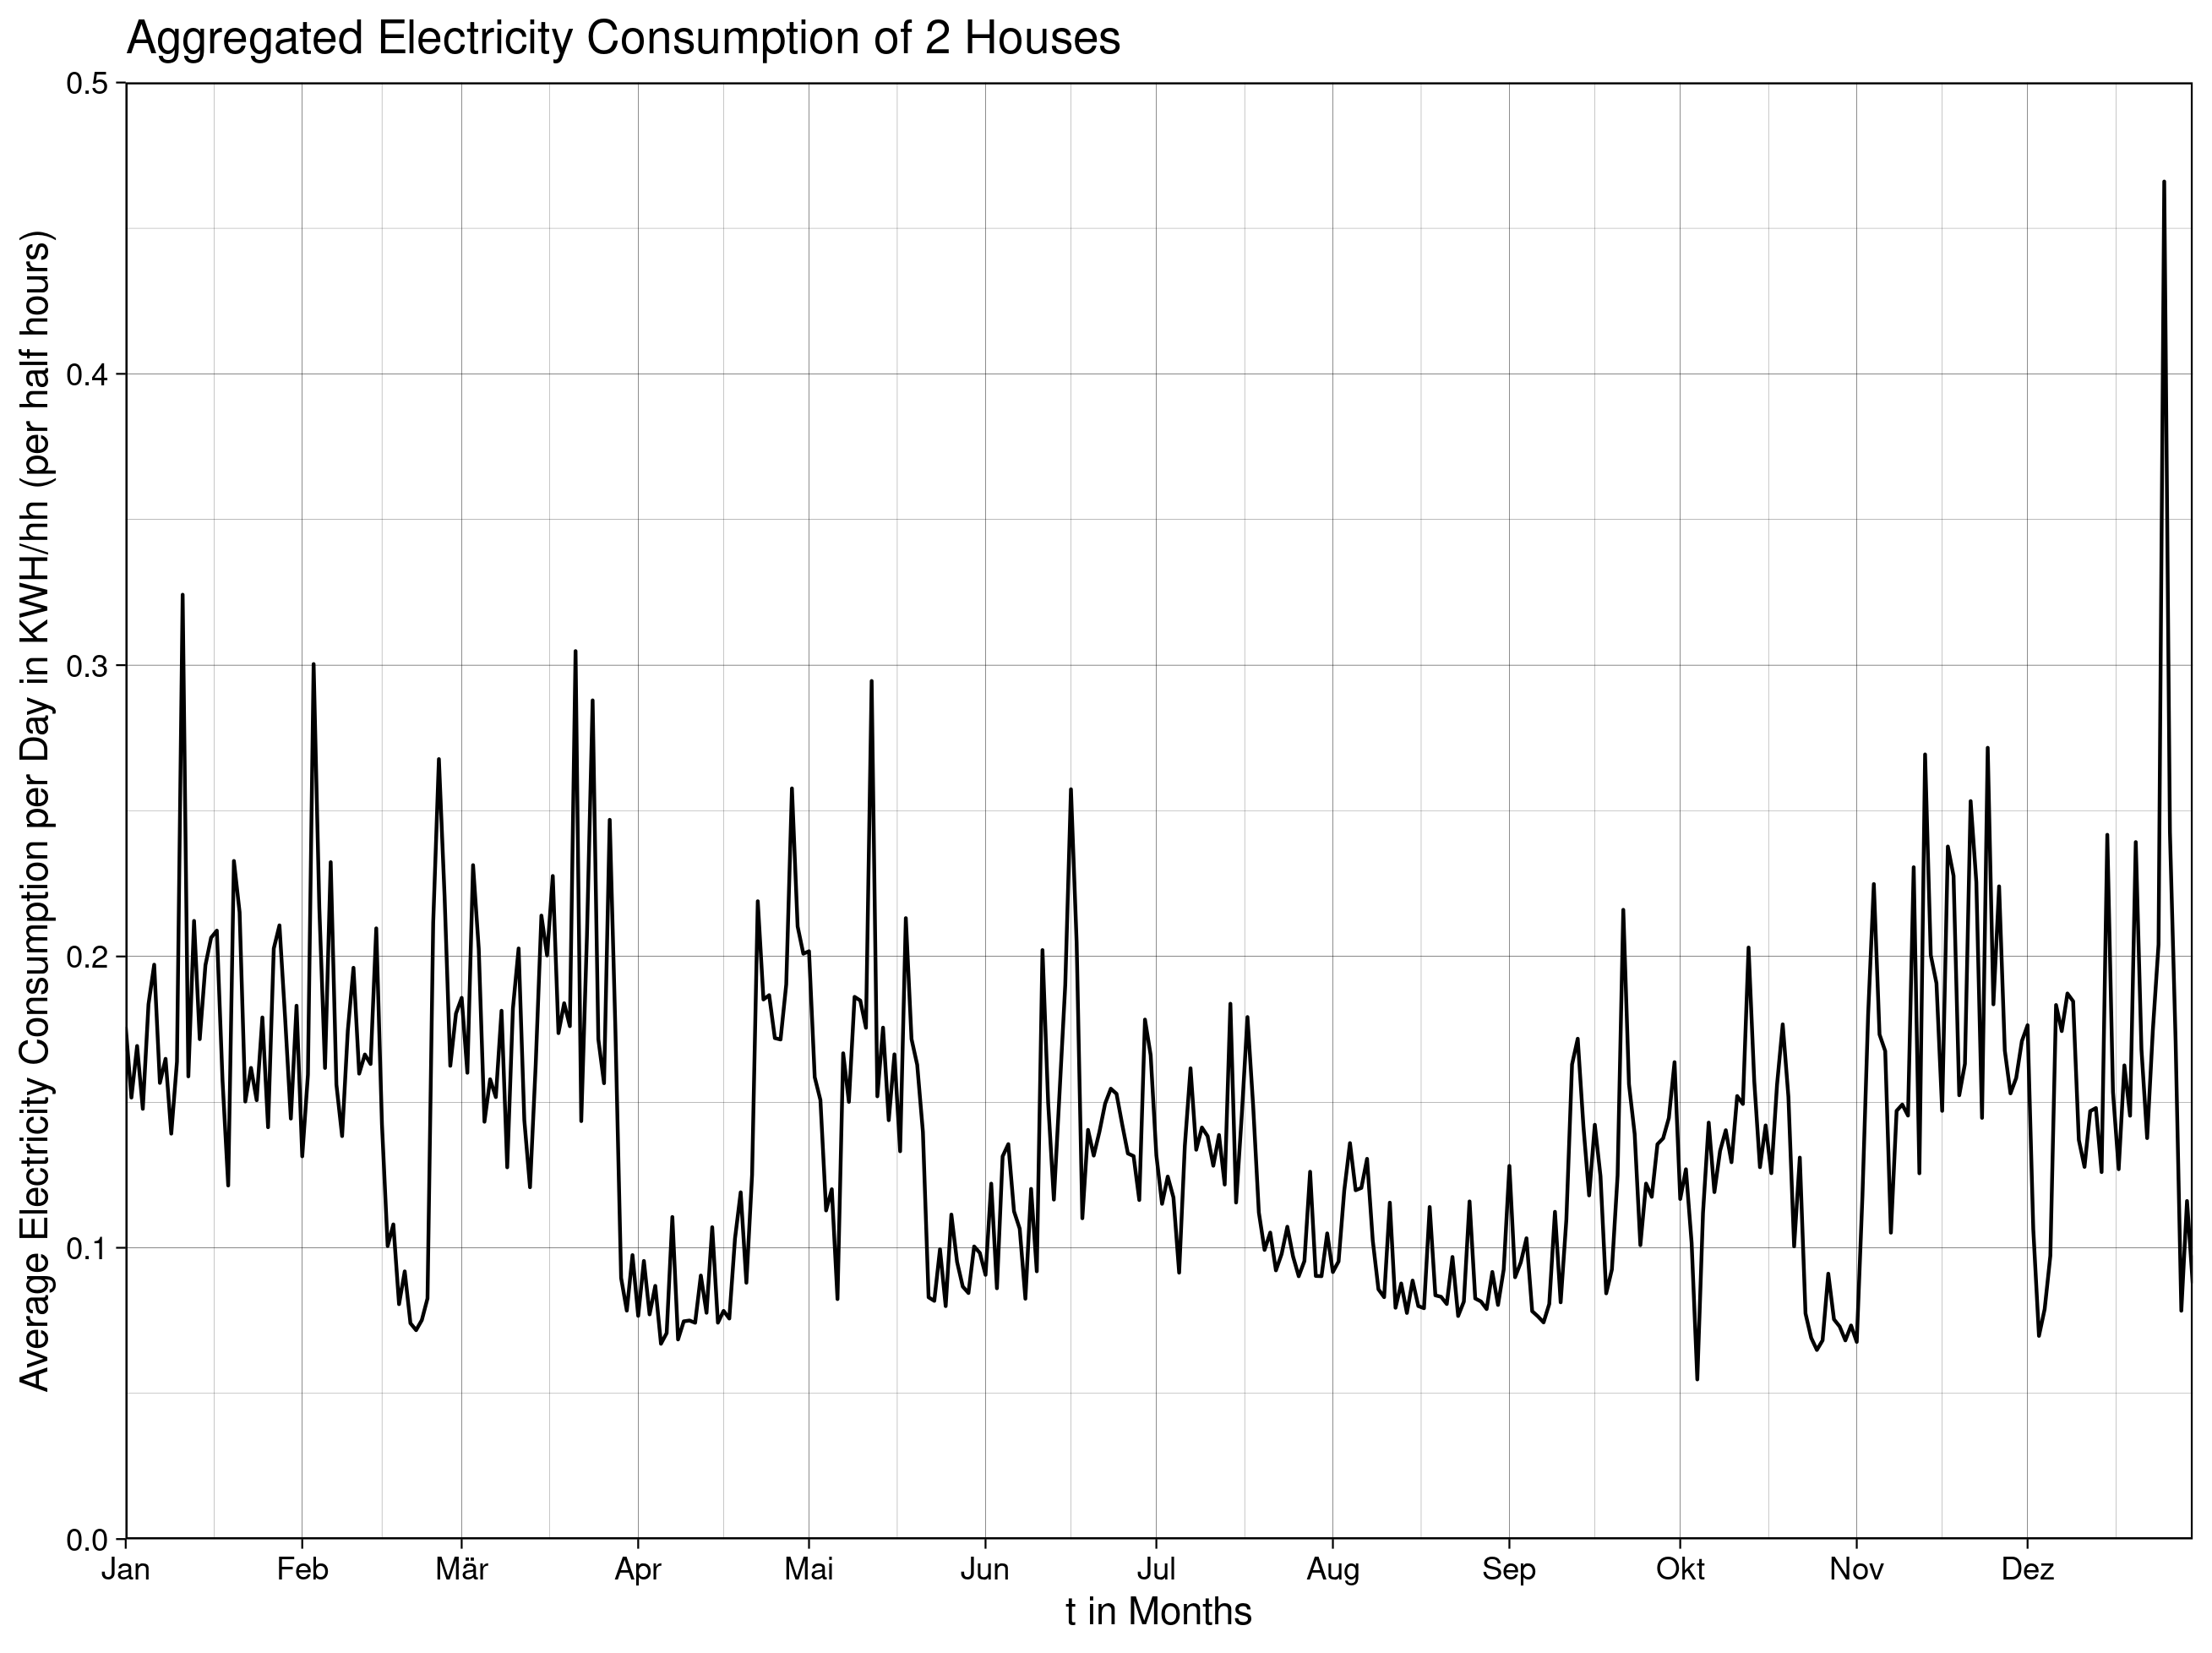
\includegraphics[width=0.85\textwidth]{images/Aggregated Electricity Consumption of 2 Houses.png}
\caption[Aggregated Electricity Consumption of 2 Houses]{}
\label{img:2_Houses}
\end{figure}
\begin{figure}[!p]
\centering
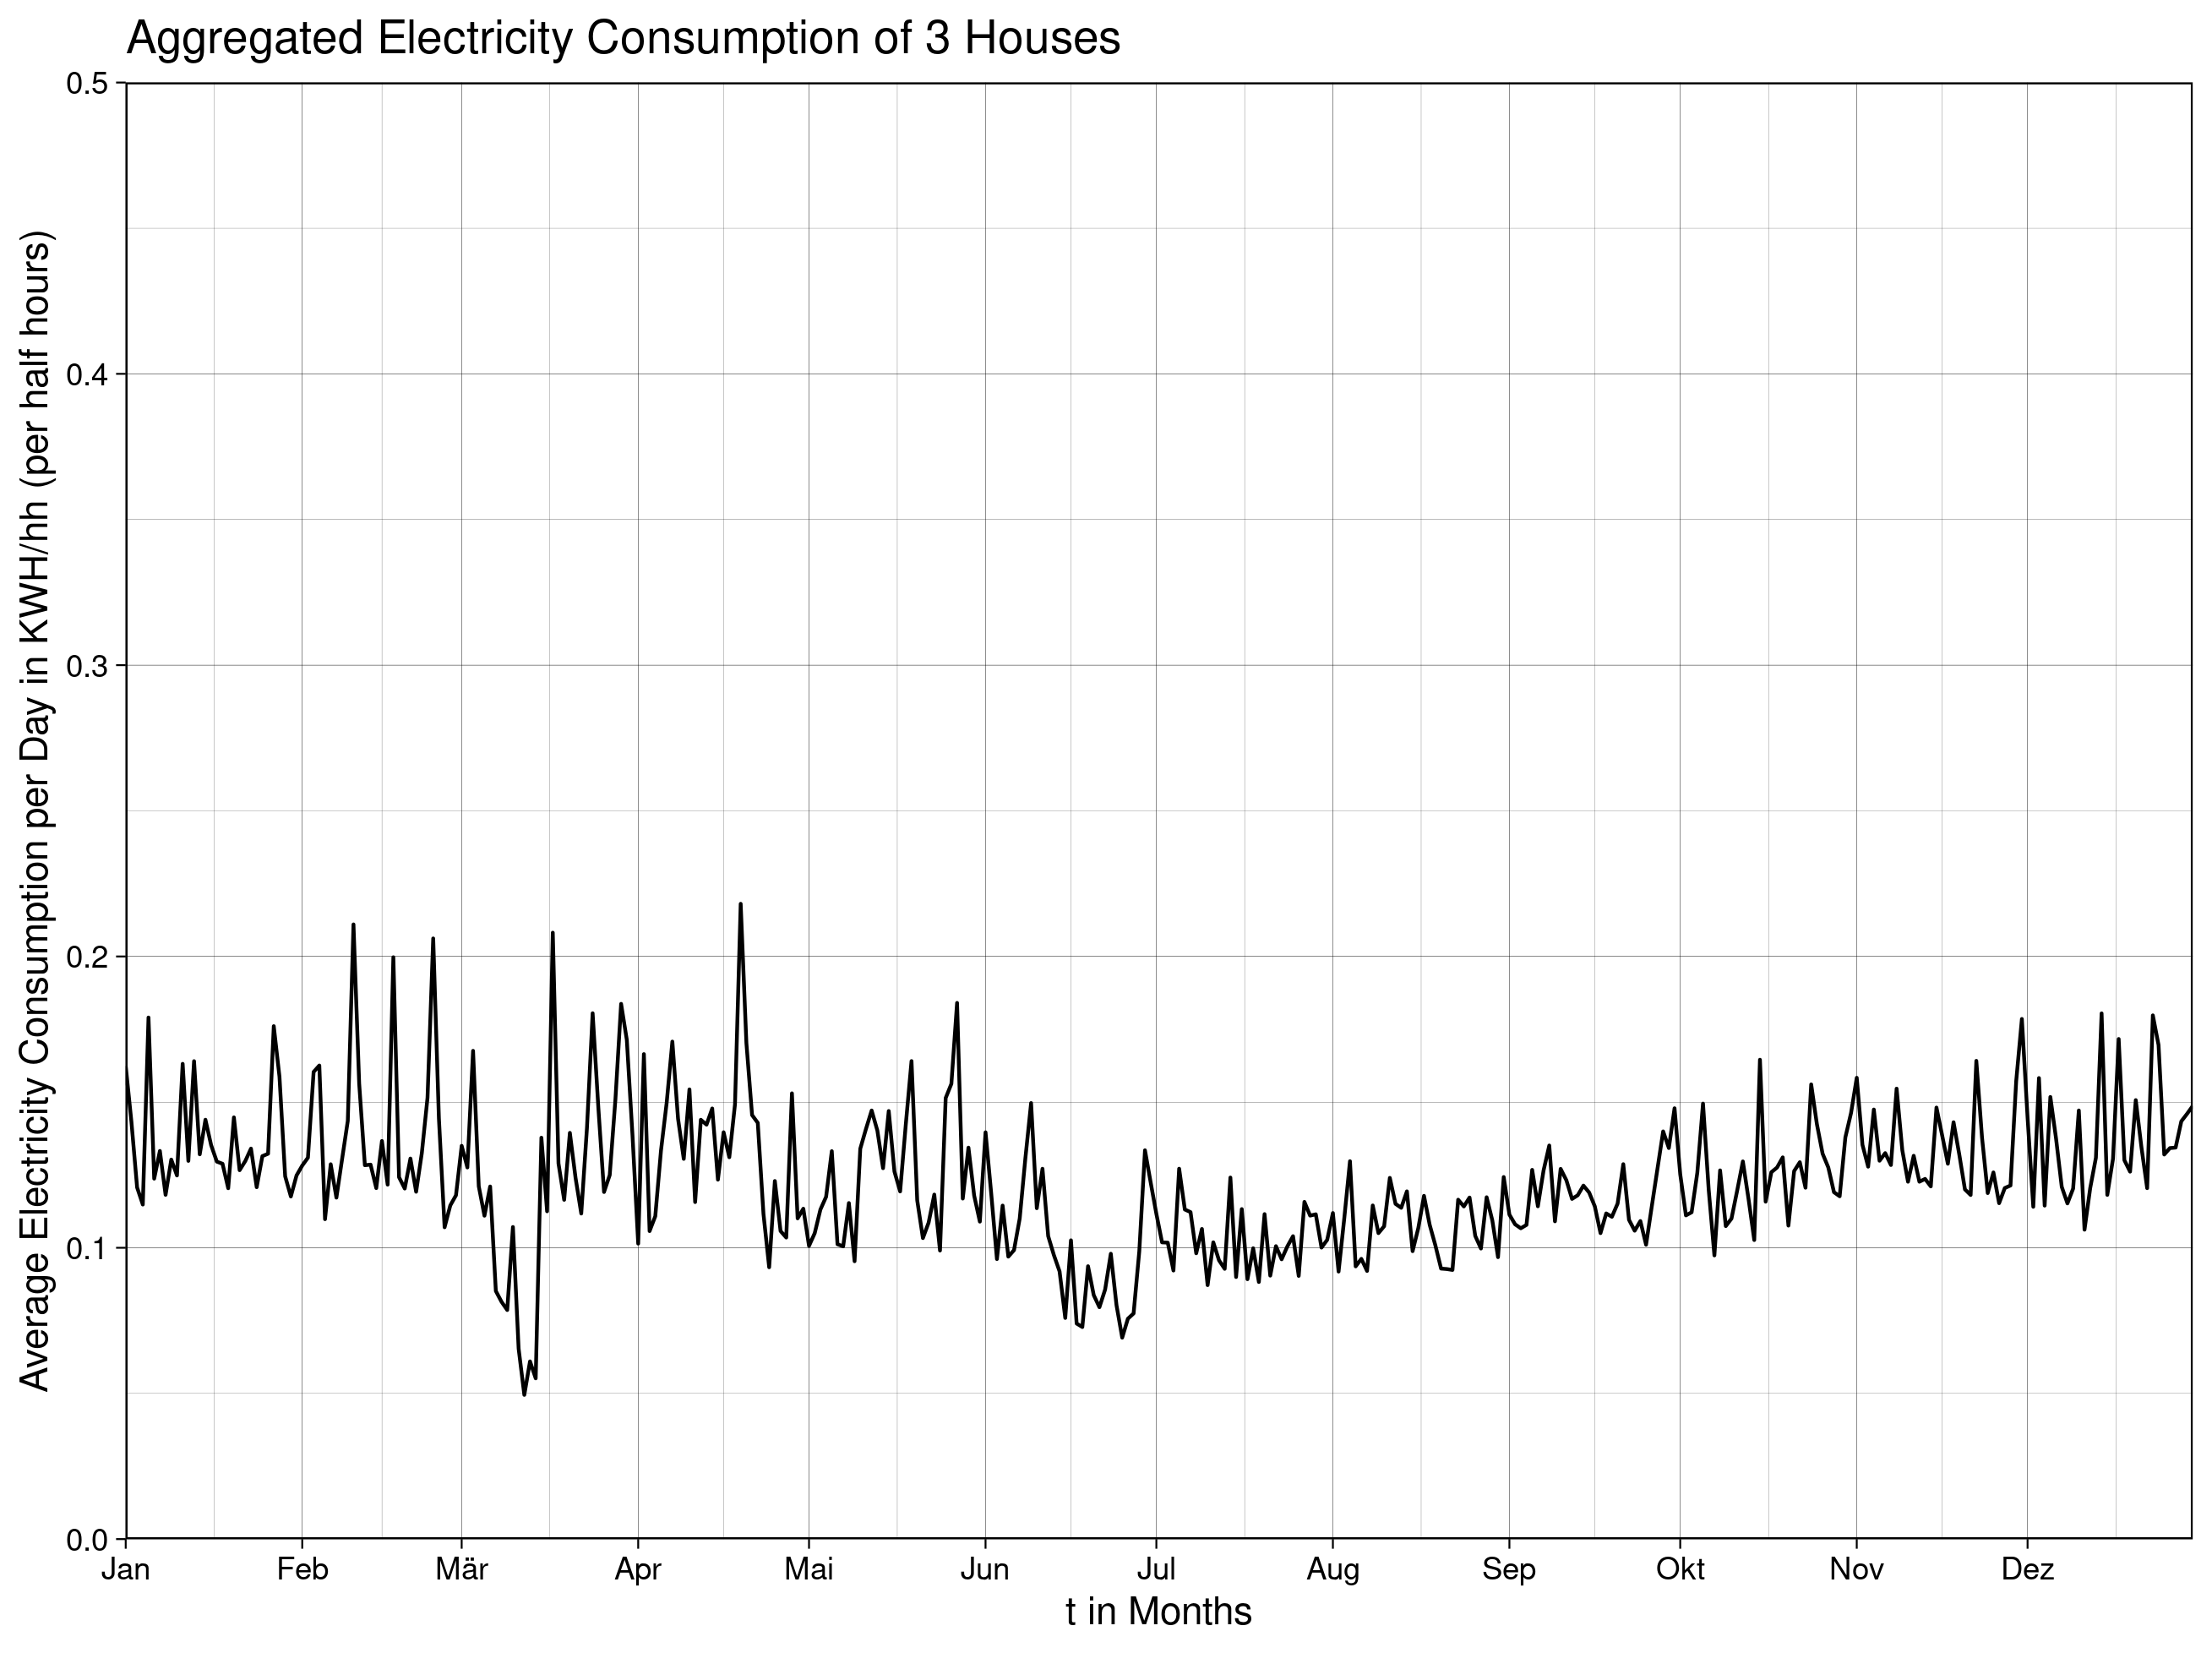
\includegraphics[width=0.85\textwidth]{images/Aggregated Electricity Consumption of 3 Houses.png}
\caption[Aggregated Electricity Consumption of 3 Houses]{}
\label{img:3_Houses}
\end{figure}
\clearpage
}
\afterpage{%
\begin{figure}[!p]
\centering
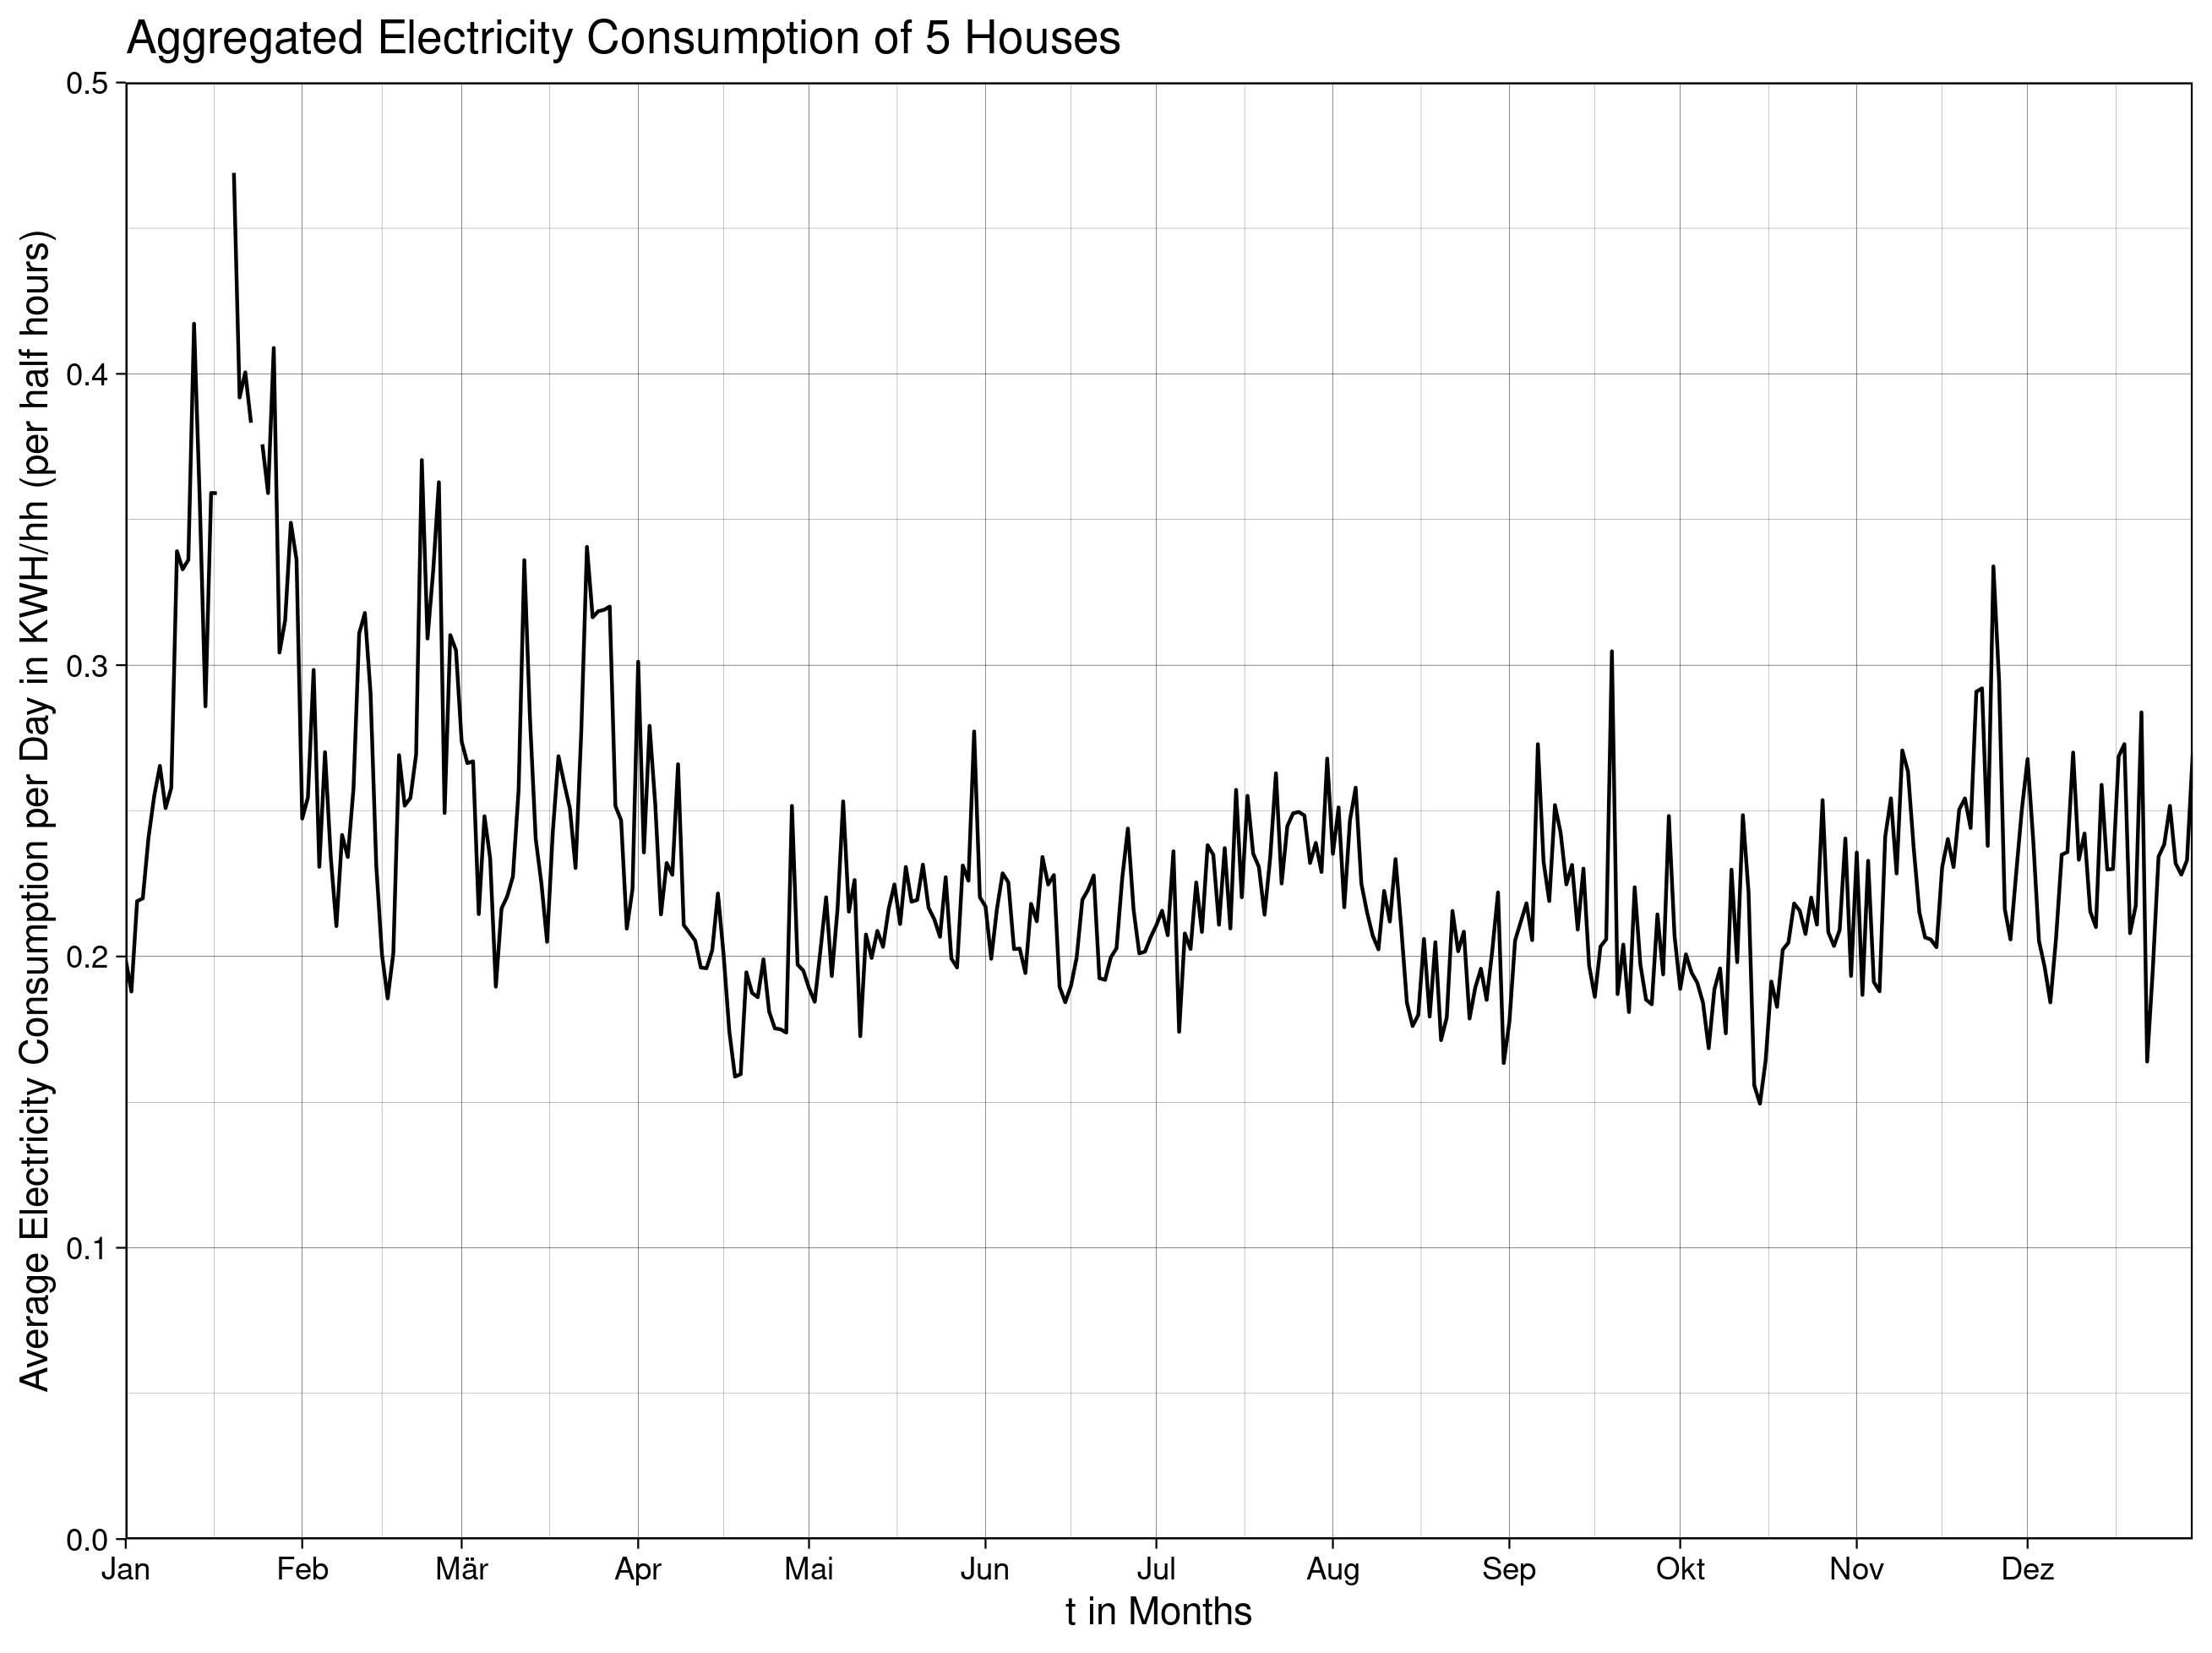
\includegraphics[width=0.85\textwidth]{images/Aggregated Electricity Consumption of 5 Houses.png}
\caption[Aggregated Electricity Consumption of 5 Houses]{}
\label{img:5_Houses}
\end{figure}
\begin{figure}[!p]
\centering
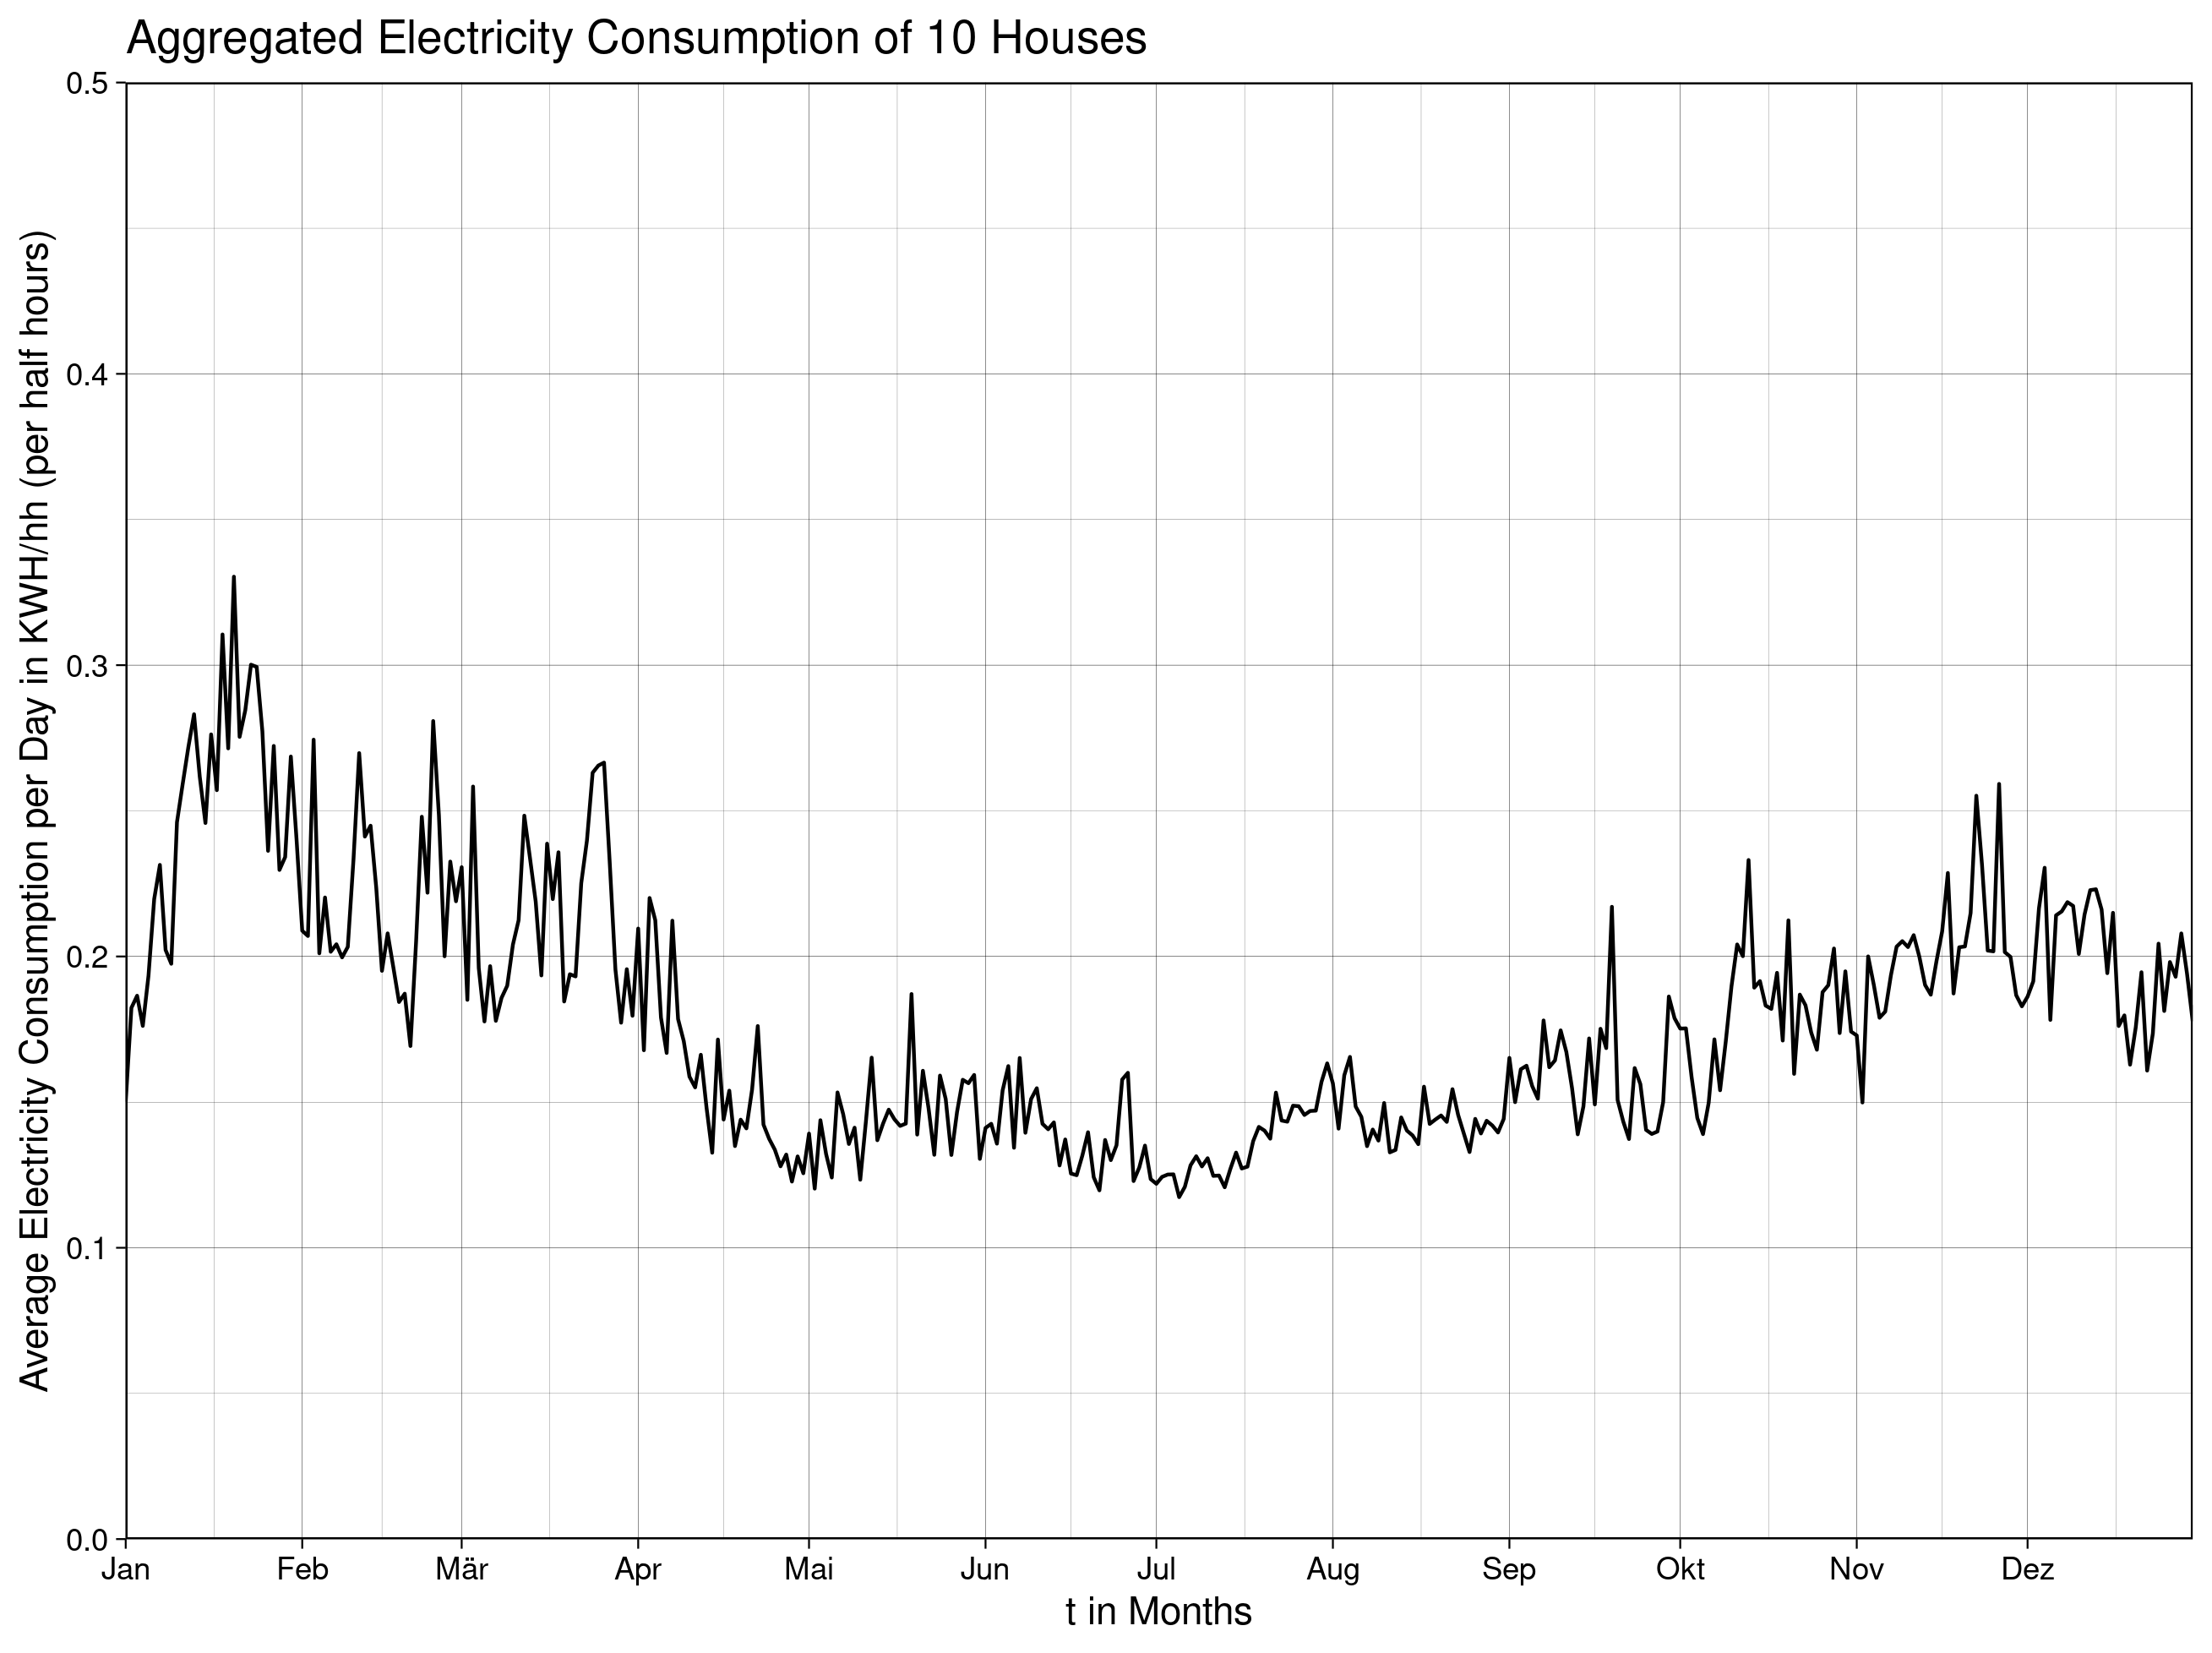
\includegraphics[width=0.85\textwidth]{images/Aggregated Electricity Consumption of 10 Houses.png}
\caption[Aggregated Electricity Consumption of 10 Houses]{}
\label{img:10_Houses}
\end{figure}
\clearpage
}
\afterpage{%
\begin{figure}[!p]
\centering
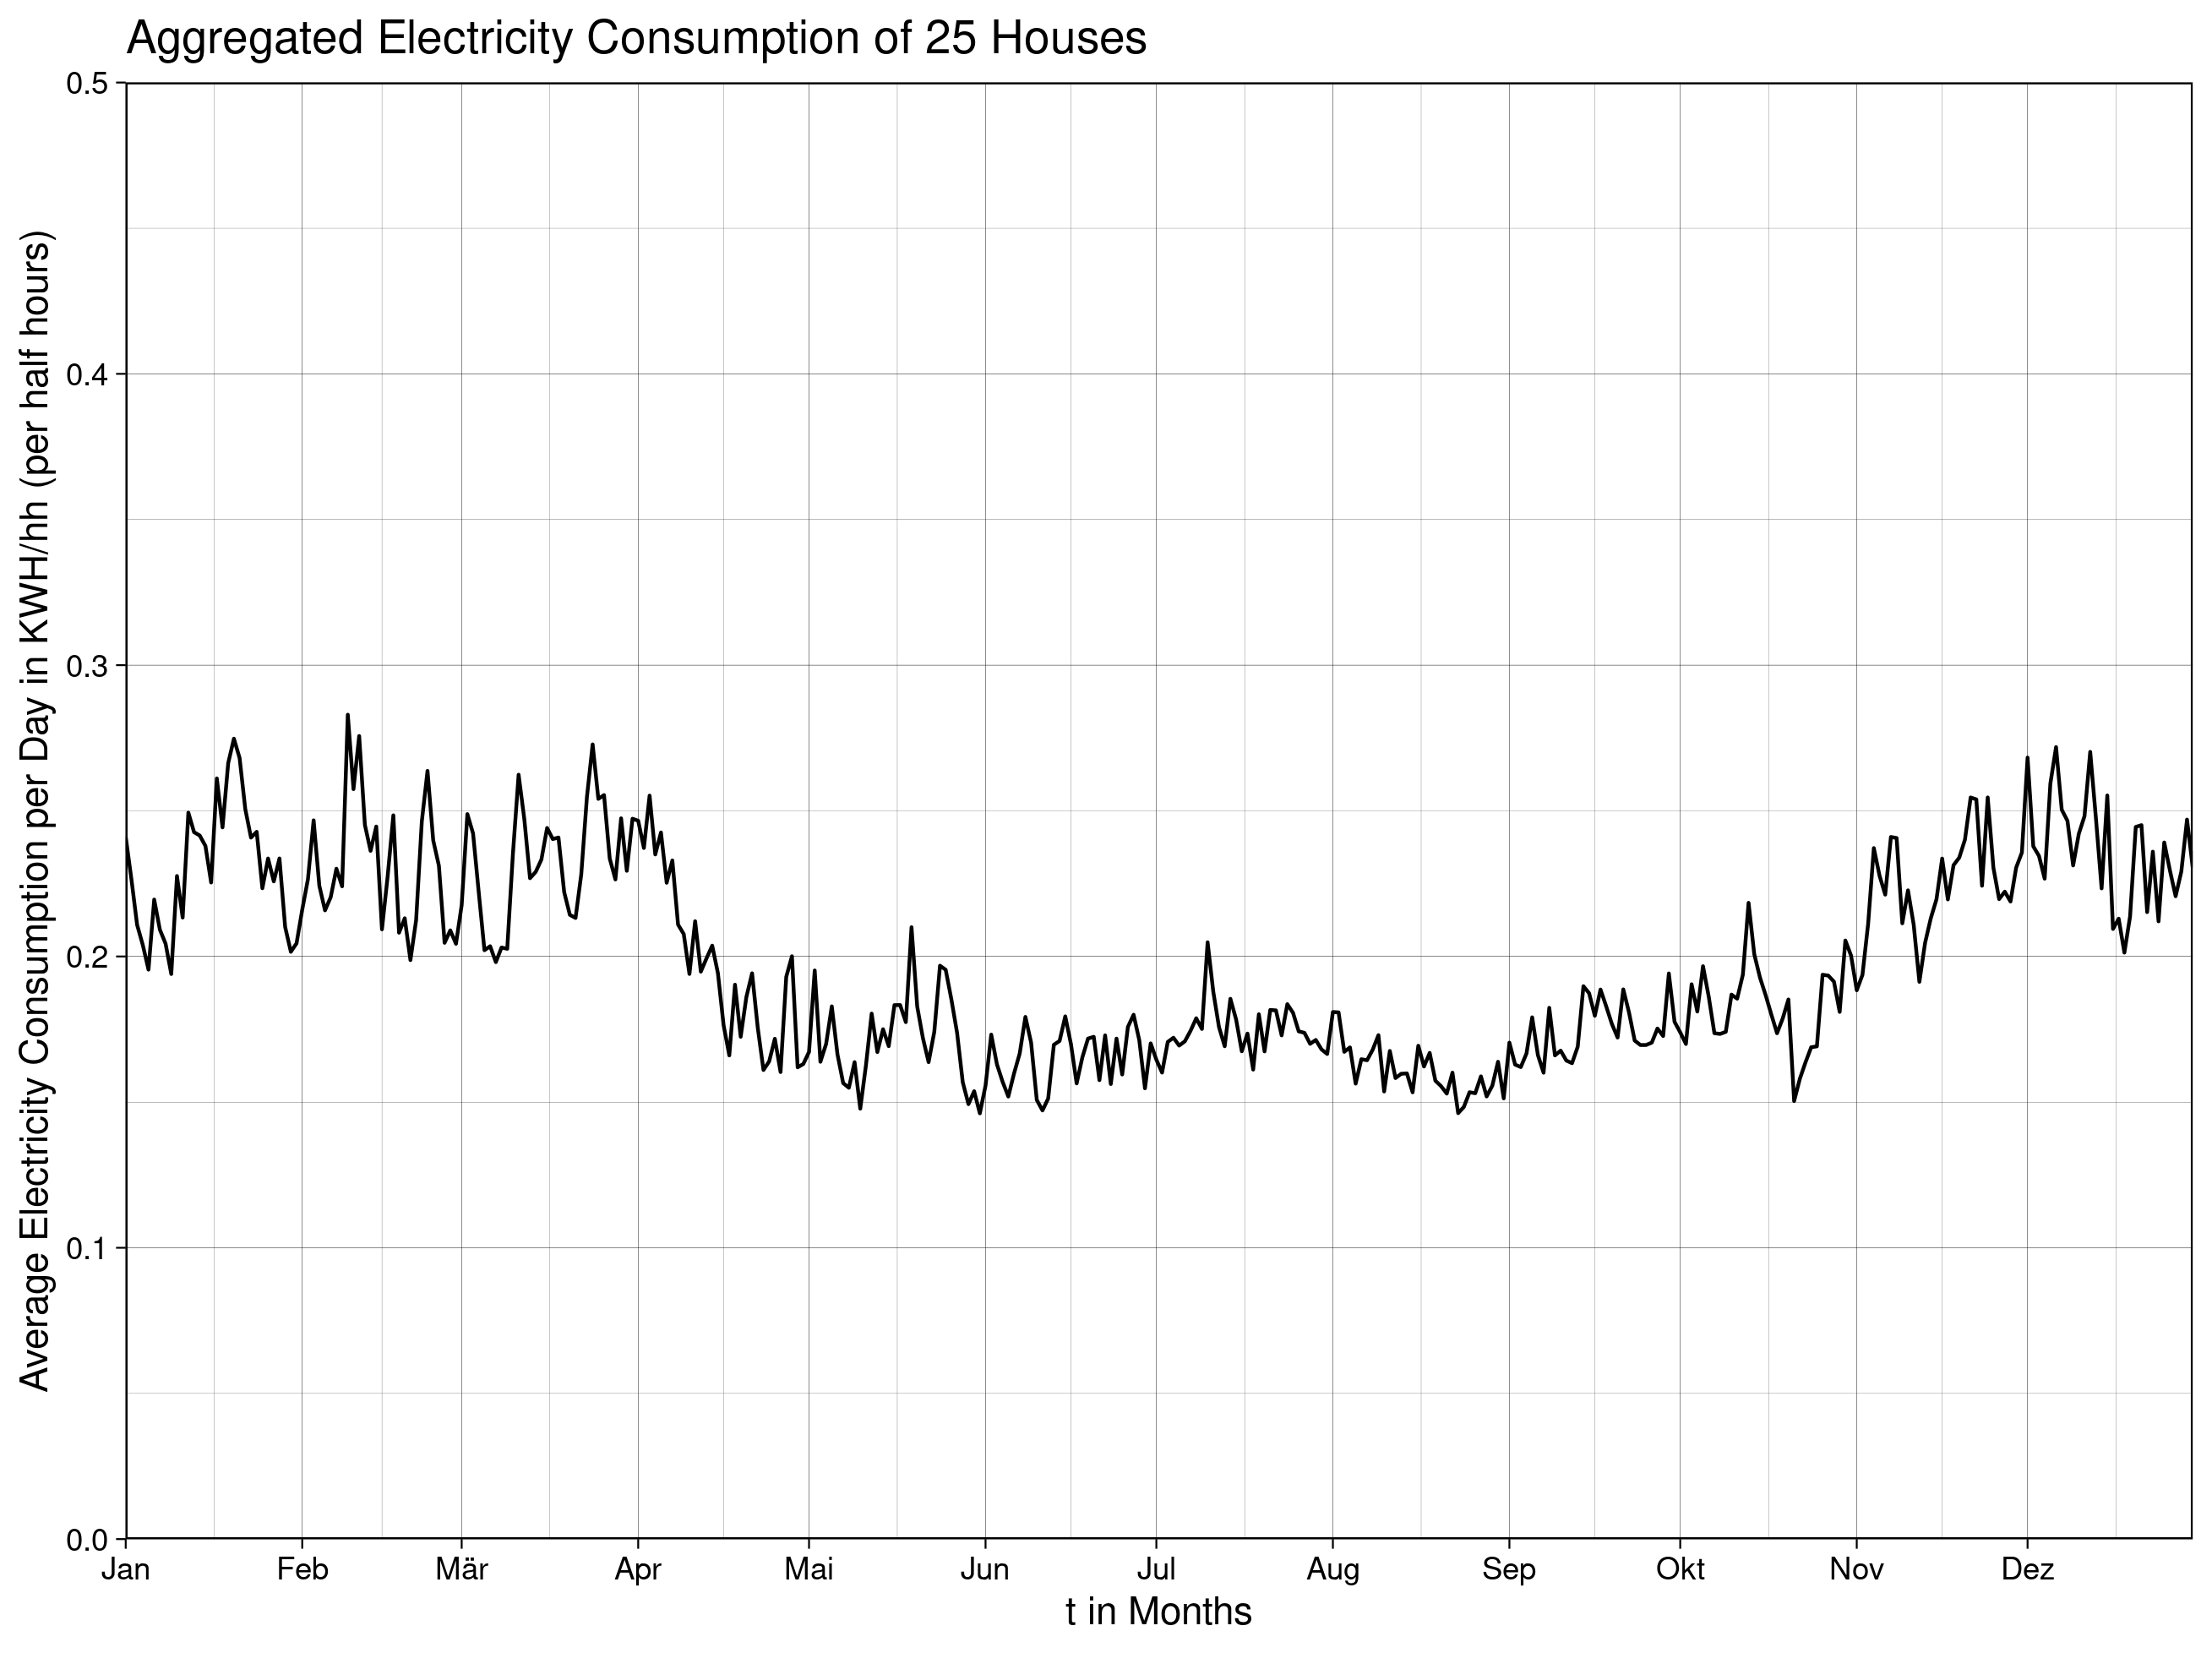
\includegraphics[width=0.85\textwidth]{images/Aggregated Electricity Consumption of 25 Houses.png}
\caption[Aggregated Electricity Consumption of 25 Houses]{}
\label{img:25_Houses}
\end{figure}
\begin{figure}[!p]
\centering
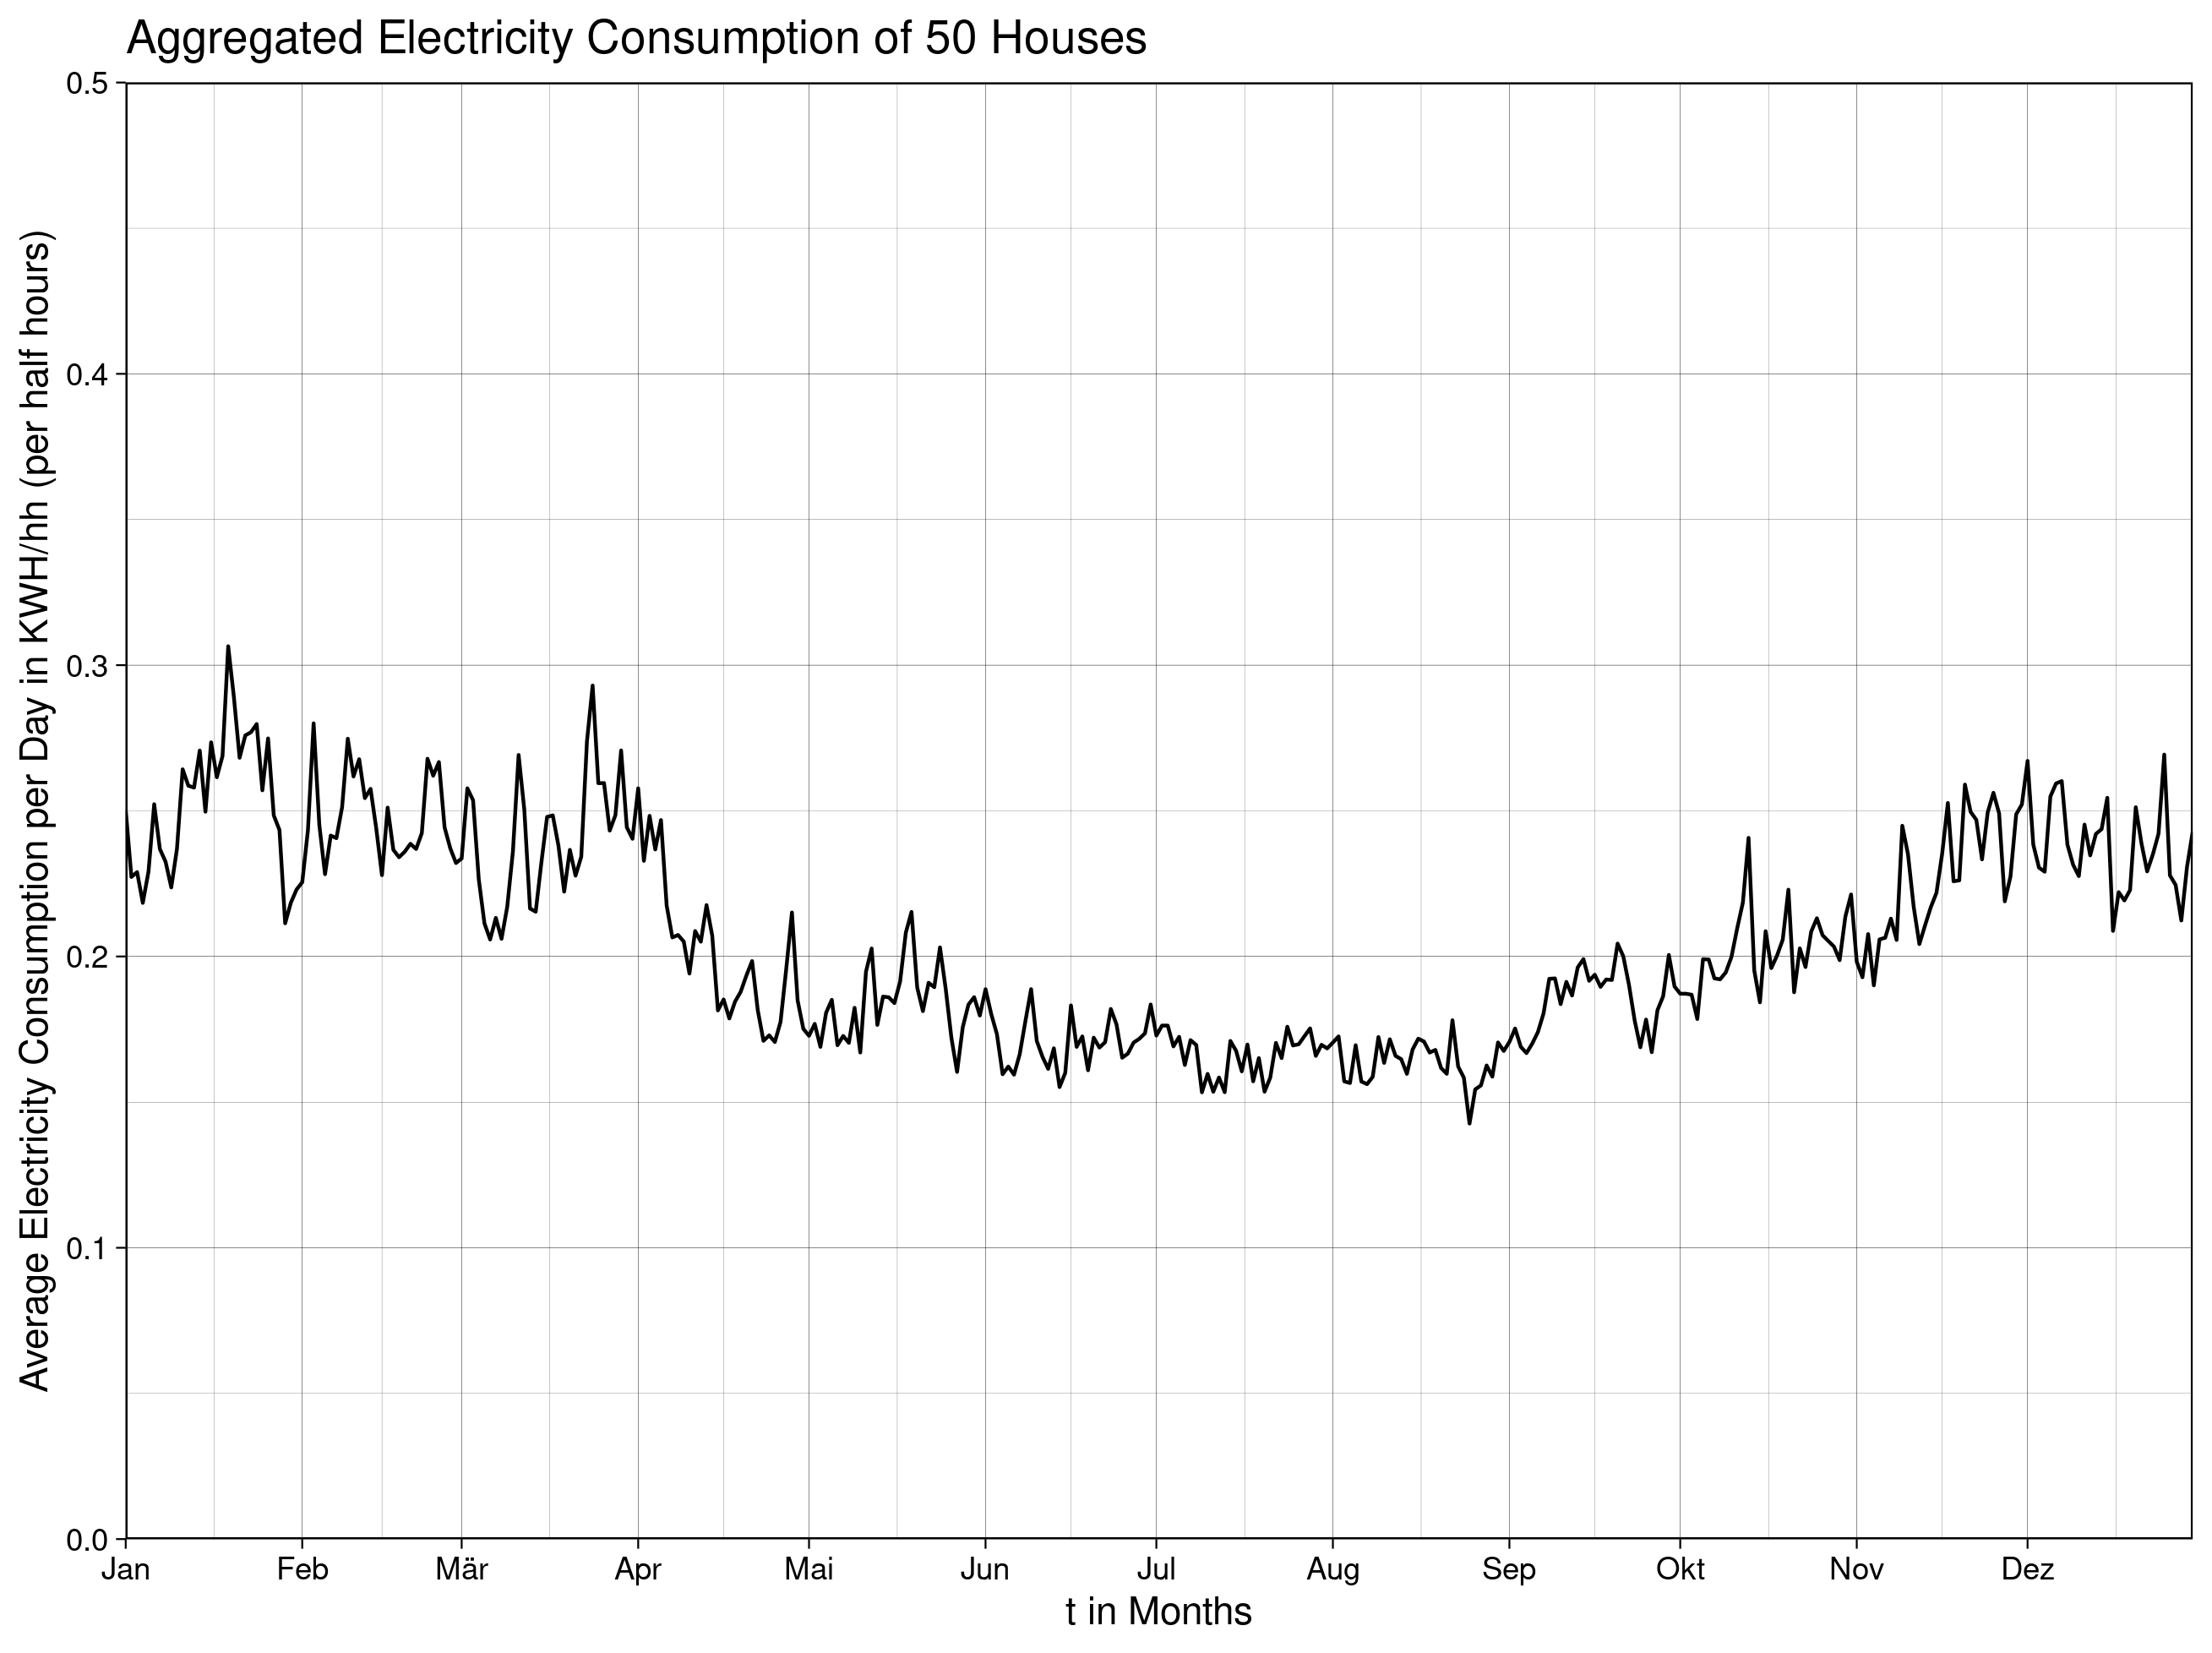
\includegraphics[width=0.85\textwidth]{images/Aggregated Electricity Consumption of 50 Houses.png}
\caption[Aggregated Electricity Consumption of 50 Houses]{}
\label{img:50_Houses}
\end{figure}
\clearpage
}
\afterpage{%
\begin{figure}[!p]
\centering
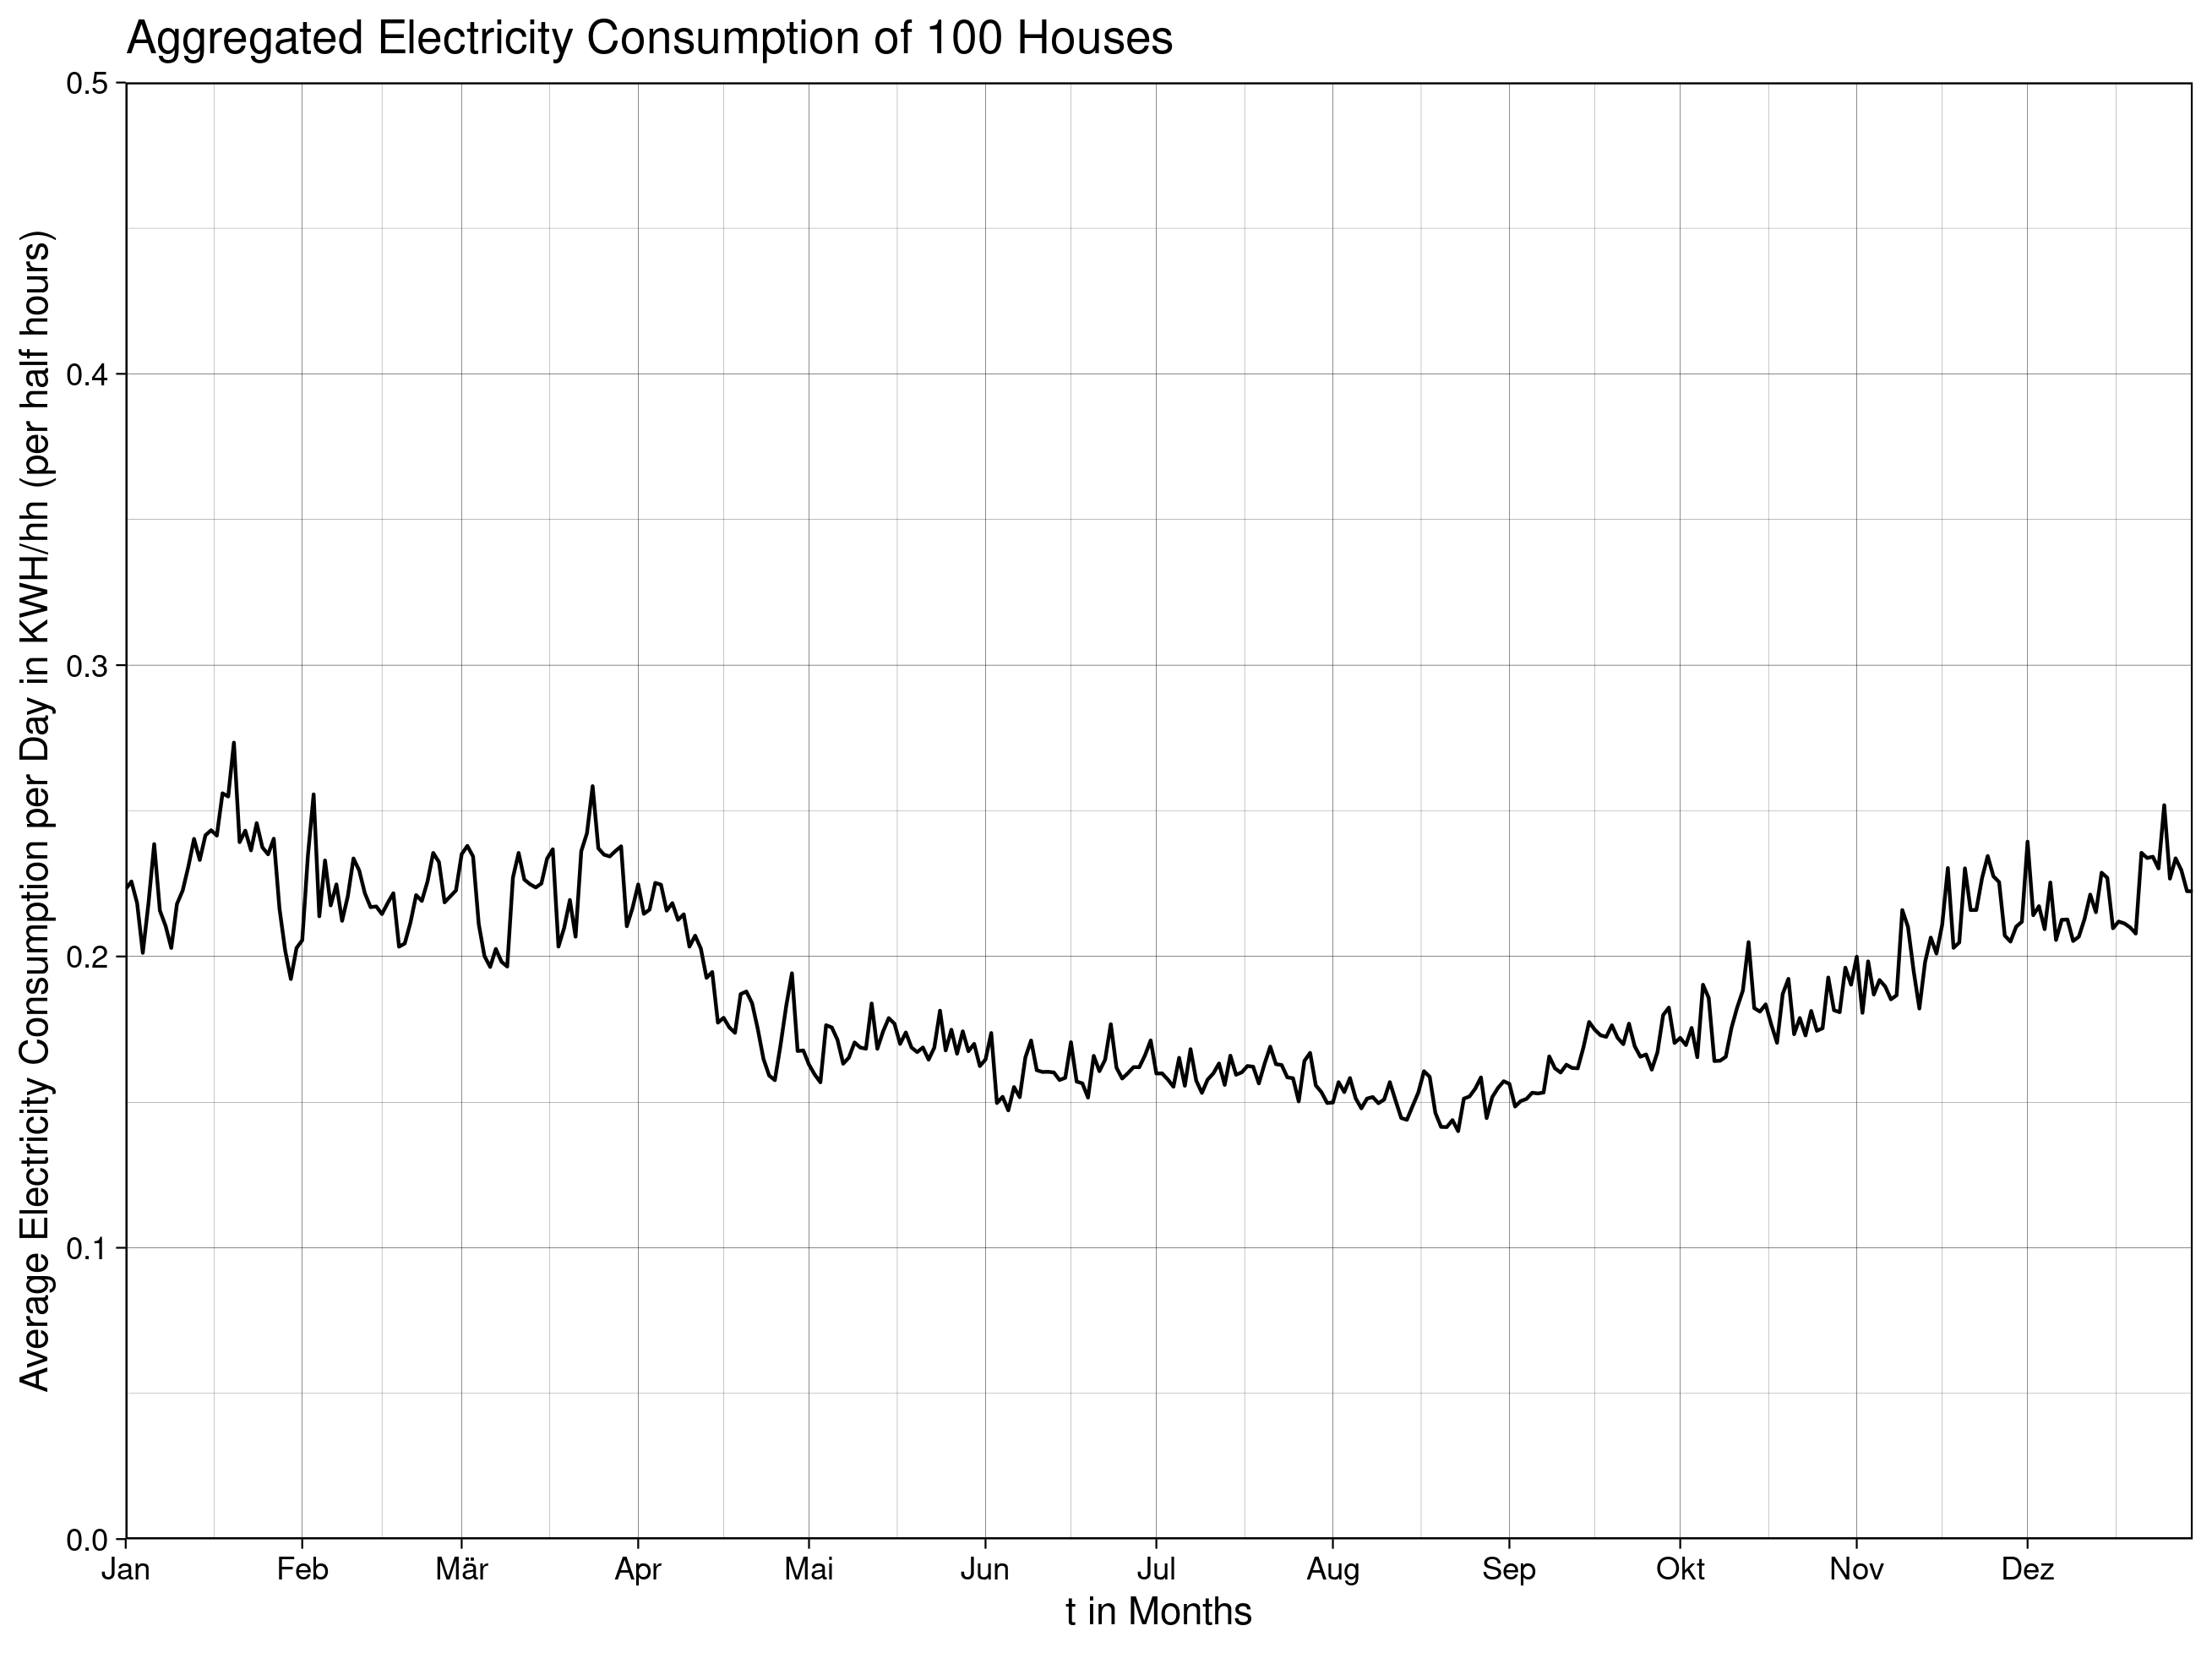
\includegraphics[width=0.85\textwidth]{images/Aggregated Electricity Consumption of 100 Houses.png}
\caption[Aggregated Electricity Consumption of 100 Houses]{}
\label{img:100_Houses}
\end{figure}
\begin{figure}[!p]
\centering
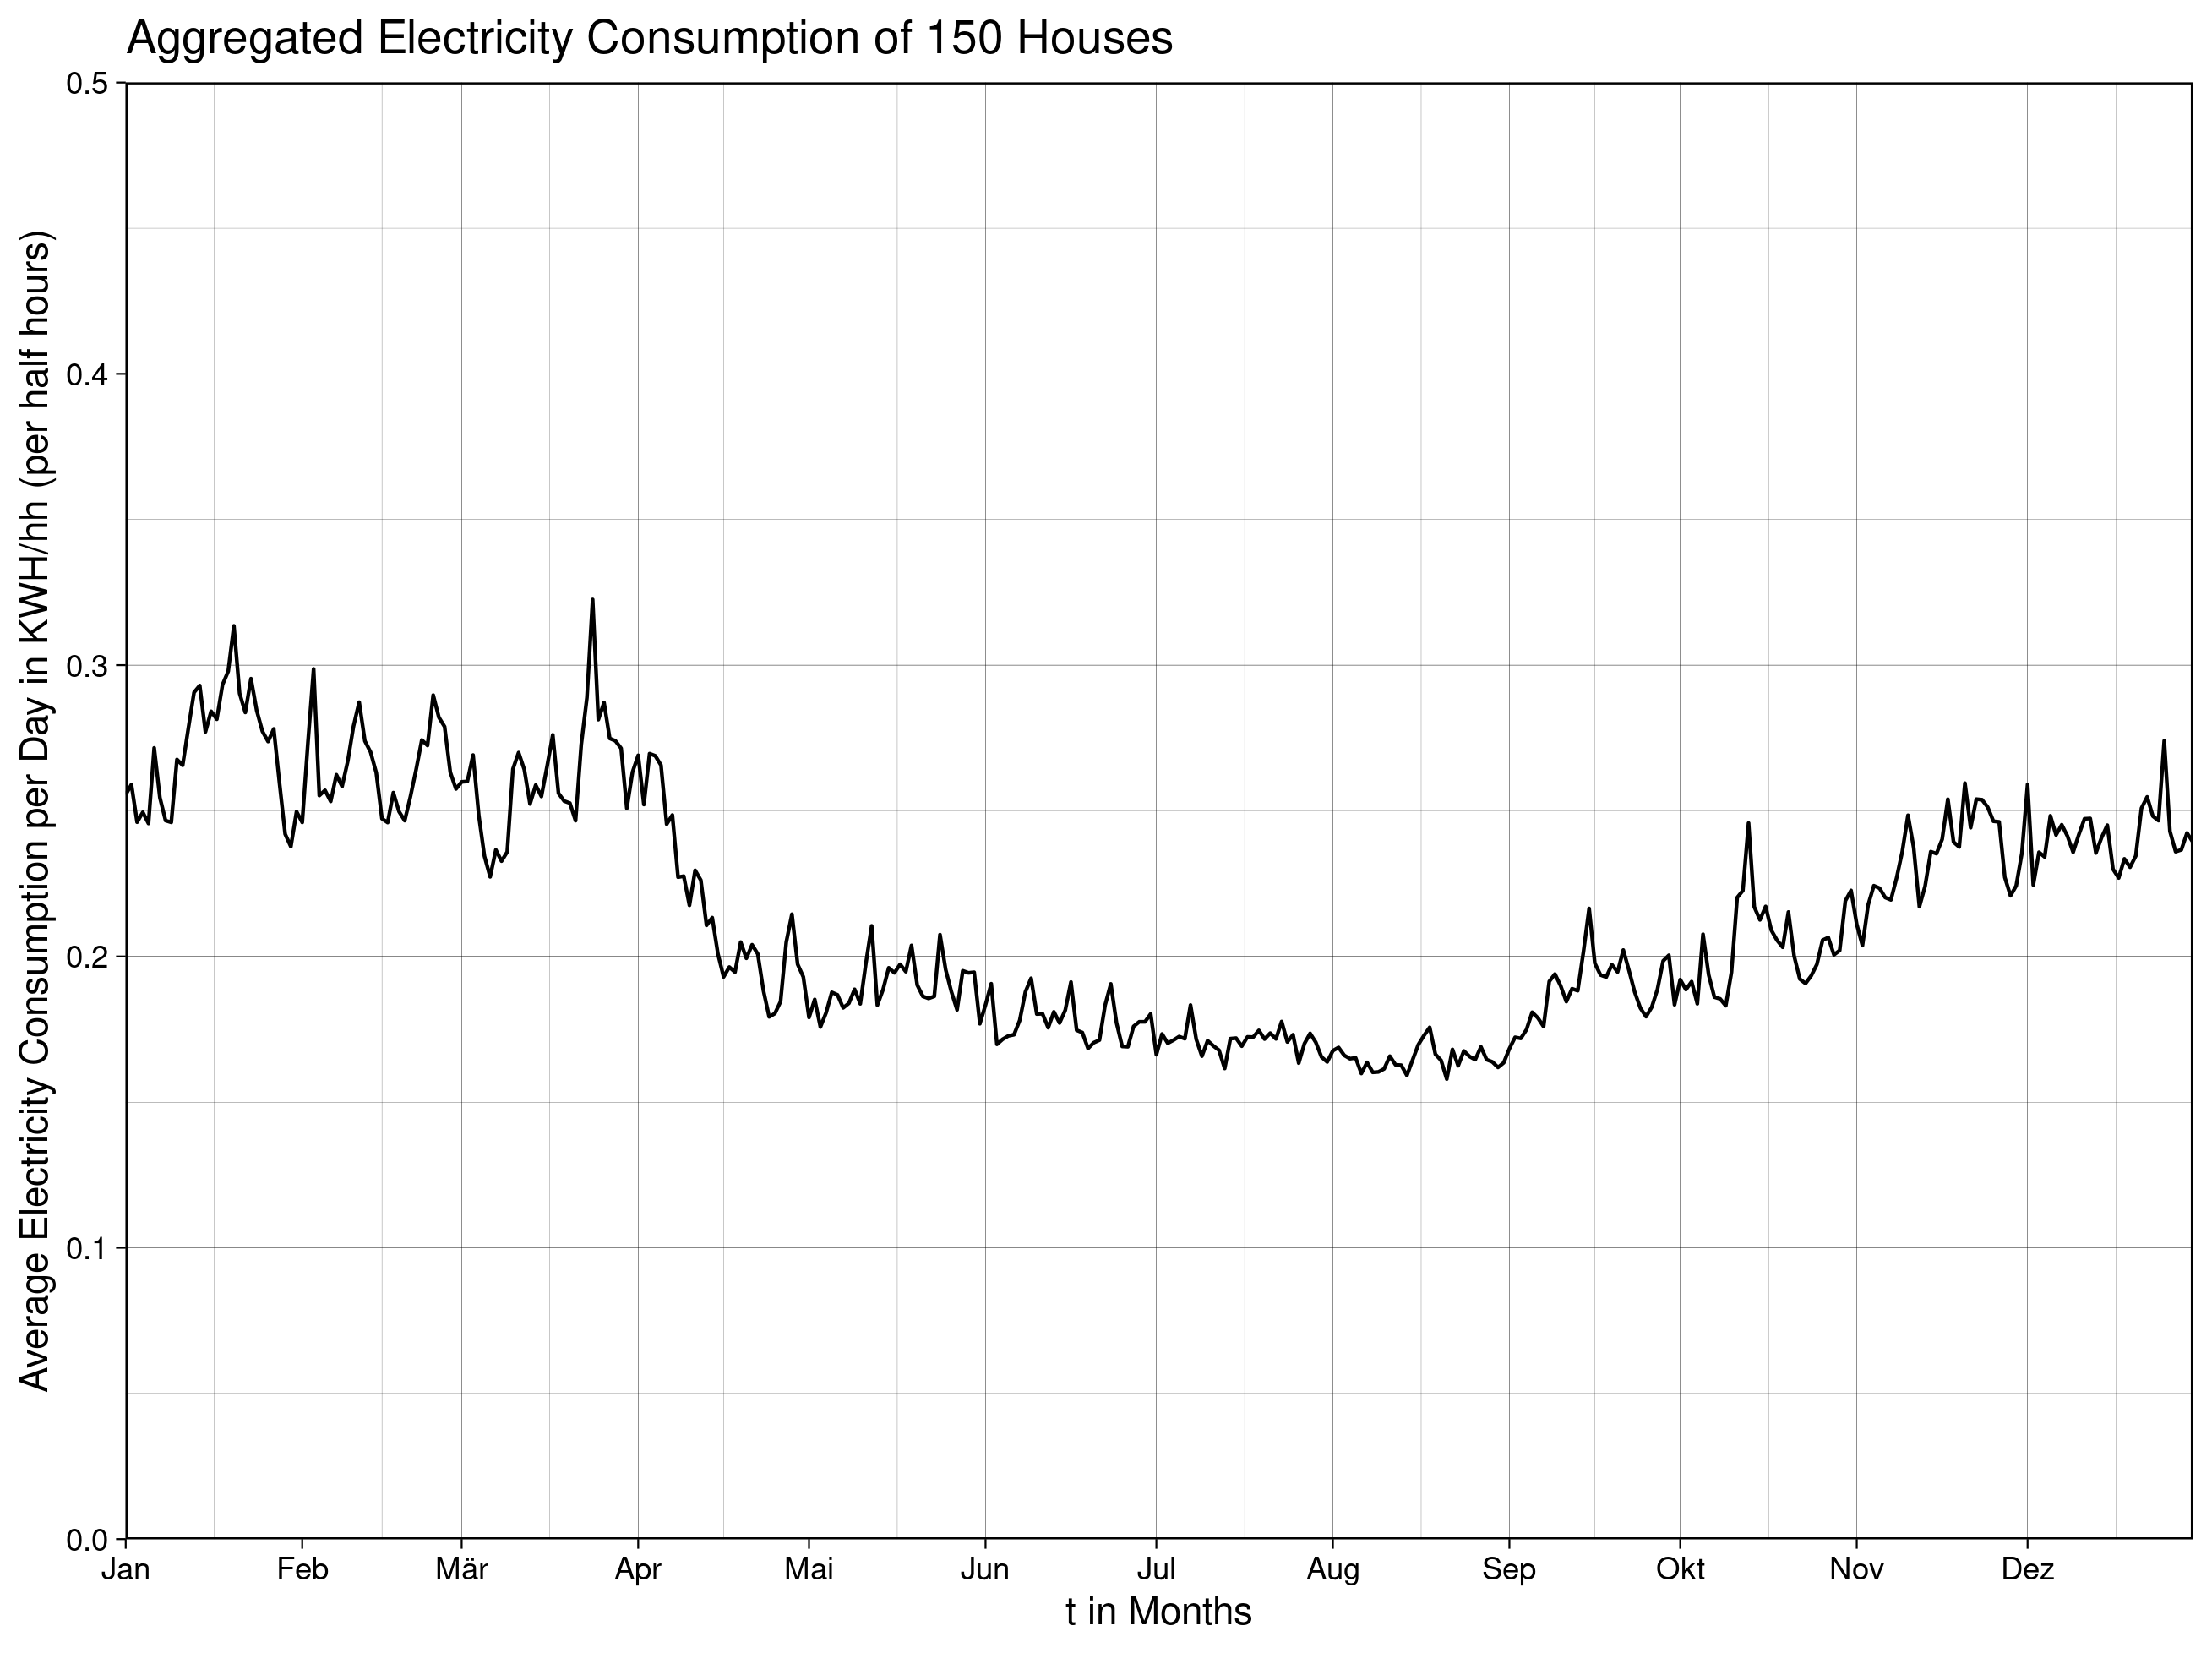
\includegraphics[width=0.85\textwidth]{images/Aggregated Electricity Consumption of 150 Houses.png}
\caption[Aggregated Electricity Consumption of 150 Houses]{}
\label{img:150_houses}
\end{figure}
\clearpage
}

\afterpage{%
\begin{figure}[!p]
\centering
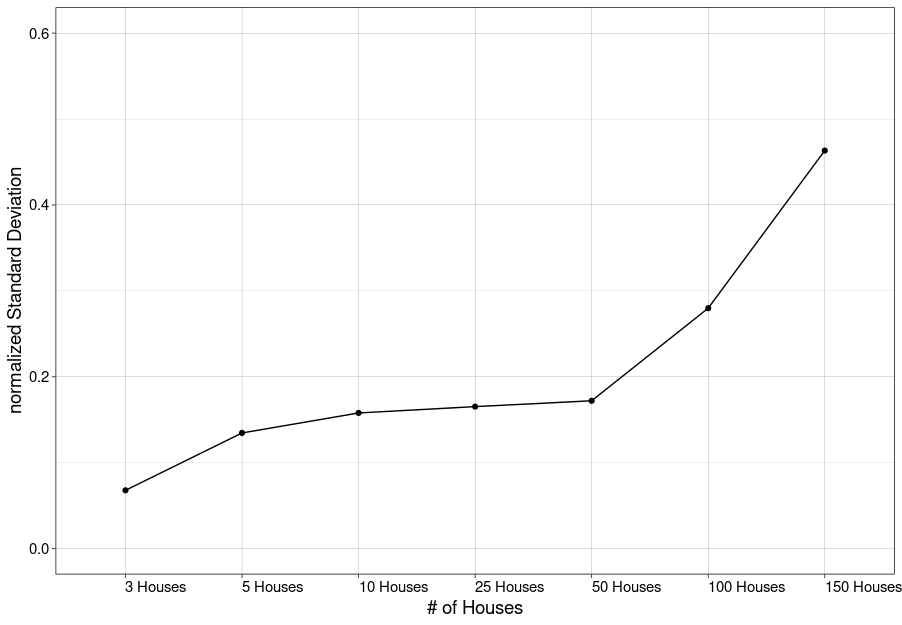
\includegraphics[width=0.85\textwidth]{images/standard_dev_test1.png}
\caption[Standard Deviation of yearlong Experiment]{}
\label{img:SD_year}
\end{figure}
\clearpage
}

